
% Dies ist der "Zentral-Dokument", die verschiedenen Teile k�nnen Sie
% unten einf�gen (s.u.). 
%
 
%[Schritgr��e, Seitenlayout, Papierformat, Satzspiegel, Bindungs-Korrektur-Ma�]
\documentclass[12pt, twoside, a4paper, DIV12, BCOR16mm]{scrartcl}

\usepackage{wrapfig, framed, caption}
\usepackage{lipsum}%

%L�ndereinstellungen
\usepackage[german,english]{babel}

%Is used with figure 
\usepackage{float}

%Math Package
\usepackage{amsmath}
\DeclareMathOperator{\atantwo}{atan2}

%Necessary to scale equations
\usepackage{graphicx}

%Wrapping figures package
\usepackage{wrapfig, blindtext}

%Mehrere Spalten
\usepackage{multicol}

%Use fig instead of Figure
\usepackage[font=small,labelfont=bf,labelsep=space]{caption}
\captionsetup{%
figurename=Fig.,
tablename=tab.,
format=plain
}

%\usepackage[english]{babel}
%Grafiken, erweiterte Kopf- und Fu�zeilen, Seienreferenzvariablen, Listings, erweiterte Symbole,
%deutsche Literatur Formatierung, zeilen-�bergreifende Kommentare, Textmarkierungen
\usepackage{graphicx, fancyhdr, lastpage, listings, wasysym, 
            bibgerm, comment, changebar} 

% weiter evtl. n�tzliche Packages: ifthen, wasysym, changebar, supertabular

%\usepackage{palatino}% weitere Schriftarten

%Color for tables
\usepackage[table,xcdraw]{xcolor}

\usepackage[latin1]{inputenc} % Umlaute richtig verarbeiten  
\usepackage[T1]{fontenc}      % Feinheiten im Satz von Umlauten

% Packages, die 'bessere' PDF-Dokumente erzeugen 
\usepackage{ae} 
\usepackage[
        pdftitle={Beispiel Thesis}
        bookmarks=true,
        bookmarksnumbered=true, % Verwendete Bookmarks anzeigen
        colorlinks,   % Farbige Links
        linkcolor=black,
        urlcolor=blue,
        citecolor=black]{hyperref}
%\usepackage[dvips]{thumbpdf}

\pagestyle{fancy}

% Legt die Einr�cktiefe der ersten Zeile f�r aller Abs�tze fest. (0:=Abs�tze nicht einr�cken)
\setlength{\parindent}{0pt}  
%\parskip1ex plus0.5ex minus0.5ex   

% Legt die Breite des Randnotizen-Bereichs festlegen (auch �ber BCORxxx konfigurierbar)
%\setlength{\marginparwidth}{25mm}
%\evensidemargin0mm
%\oddsidemargin8mm

% Definiert die Gesamth�he des Textrumpfes f�r alle nachfolgenden Seiten.
\setlength{\textheight}{225mm}
\setlength{\headheight}{13mm}
\setlength{\topskip}{10mm}

% Nummerierungstiefe des Inhaltsverzeichnis 
\setcounter{tocdepth}{2} % auch {3} ist OK aber bitte nicht mehr

% Kopfzeilenformatierung
%\fancyhead[RO,LE]{\small \sffamily Inhalt} 
%\fancyhead[LO,RE]{\small \sffamily Beispiel f�r ein \LaTeX\ Dokument} 


%
% texAbbrev.tex: Einige Abk�rzugen 
%

\newcommand{\ia}{i.\,Allg.\ }
\newcommand{\dht}{d.\,h.\ }
\newcommand{\ua}{u.\,a.\ }
\newcommand{\so}{s.\,o.\ }
\newcommand{\zb}{z.\,B.\ }
\newcommand{\zbdp}{z.\,B.:\ }
\newcommand{\idr}{i.\,d.\,R.\ }
\newcommand{\zt}{z.\,T.\ } 
\newcommand{\zz}{z.\,Zt.\ } 
\newcommand{\igs}{i.\,Ggs.\ } 

\newcommand{\code}{\ttfamily}

\newcommand{\svs}{\vspace*{0.5ex}} 
\newcommand{\myrule}{\ \vspace{1ex} \\ \hrule} 
\newcommand{\figref}[1]{Fig.~\ref{#1}} 
\newcommand{\secref}[1]{Section~\ref{#1}} 
\newcommand{\mymargin}[1]{\marginpar{\raggedright \footnotesize \sffamily #1}} 

\renewcommand{\topfraction}{0.95}
\renewcommand{\bottomfraction}{0.95}

\newenvironment{trilist}{
    \renewcommand{\labelitemi}{\(\triangleright\)}
    \renewcommand{\labelitemii}{{\bfseries -}}
    \setlength{\partopsep}{0ex plus .5ex minus .5ex} 
    \setlength{\topsep}{-1ex plus .5ex minus .5ex} 
    \setlength{\parskip}{1.2ex plus .5ex minus .5ex}
    \setlength{\itemsep}{0pt plus .5ex minus .5ex}
    \setlength{\parsep}{0pt plus .5ex minus .5ex} 
    \begin{itemize}
    }
   {\end{itemize}}

 % eigene Kommandos laden 


\begin{document} 
\selectlanguage{english}

\includecomment{comment}
\excludecomment{unsinn1} % ben�tigt das Package "comment". Ein- und Auschalten von Textteilen z.B. Anmerkungen 
\begin{unsinn1} 
Hier steht ein unsinniger Text, welcher aber gl�cklicher Weise nicht angezeigt wird!!!
\end{unsinn1} 

%Titelseite
\begin{titlepage}
\sffamily
\setlength{\tabcolsep}{0mm}
\begin{tabular*}{\textwidth}{l@{\extracolsep\fill}r} 

%\hspace{-0.4cm}
%
\includegraphics[width=6cm]{Bilder/logo_welle_en}  % Englische Version des Logos 

\includegraphics[width=5cm]{Bilder/rwu} % Deutsche Version des Logos

  &
\raisebox{3mm}{
	\begin{tabular}{r}
%\rule{0cm}{0.5cm}
Course Applied Computer Science\\[0.5mm]
School of Electrical engineering and Computer Science\\
\end{tabular}}
\end{tabular*}
\setlength{\tabcolsep}{6pt}

\vspace*{4cm}
\begin{center}
\textbf{\Large{Bachelor-Thesis}}\\
\vspace*{1cm}
\textbf{\LARGE{Self-Supervised Machine Learning Pipeline for Obstacle Avoidance}}\\
\vspace*{2cm}
\large{for the purpose of obtaining the degree}\\[2mm]
\large{Bachelor of Computer Science}\\
\end{center}

%\vfill
\vspace{2cm}
\begin{center}

	submitted by:\\[5mm]
{\Large Martin Samuel Lanz} \\[5mm]
    \today \\[3cm]
{\normalsize
	\begin{tabular}{rl}
	1. Gutachter: 	& Prof. Dr. Markus Schneider\\
	2. Gutachter: 	& M.Sc. Daniel Hofer 
	\end{tabular}
}
\end{center}

\end{titlepage}


%Eidesstattliche Erkl�rung
\begin{newpage}
\vspace*{\fill}
\section*{Eidesstattliche Erkl�rung}
Hiermit versichere ich, die vorliegende Arbeit selbststndig und unter ausschlielicher Verwendung der angegebenen Literatur und Hilfsmittel erstellt zu haben. Die Arbeit wurde bisher, in gleicher oder hnlicher Form, keiner anderen Prfungsbehrde vorgelegt und auch nicht verffentlicht.\\\\

\vspace{3cm}
\begin{tabular*}{\textwidth}{c@{\extracolsep\fill}cc}
\cline{1-1}
\cline{3-3}
\\
\ \ \ \ \ \ \ \ \ Unterschrift\ \ \ \ \ \ \ \ \ \ & & \ \ \ \ \ \ \ \ \ Ort, Datum\ \ \ \ \ \ \ \ \ \\
\end{tabular*}
\end{newpage}



%Vorwort, Zusammenfassung(Abstract), Danksagung(Acknowledgements)
\begin{newpage}
\vspace*{\fill}
\section*{Abstract}
This Bachelor thesis proposes a self-supervised Machine Learning pipeline for obstacle avoidance, where a 2-dimensional image serves as the input, and a laser provides the relevant ground truth necessary for training.\\

Self-supervision has the advantage that no human labeling is necessary to gather data for training. The project will show that this is possible with a simple camera and a laser and refer to other projects with similar approaches.\\

The goal is further to implement as many pieces of a machine learning pipeline, as autonomous as possible, where a user can start a robot in a given environment, gather data, use that data for training, and then operate on the deployed model.\\

I have chosen this topic, not because of merely personal interests in machine learning, but also as an addition to our area of specialization and as an extension to previous classes like Autonomous Mobile Robots or Artificial Intelligence.\\

\section*{Acknowledgments}
Throughout the writing of this thesis, I have recevied a great deal of support and assistance.\\

I would first like to express my gratitude to Mr. Daniel Hofer M.Sc, and Mr. Benjamin St�hle M.Sc., who constantly gave me excellent support and advice along this project.\\

I would also like to thank my first supervisor, Professor Dr. Markus Schneider, for his suggestions and support.\\

I also want to thank my father, for his great support. Without him, it would have been much more challenging or even impossible, to study and organize everything which comes along, while I could focus on school.\\

Furthermore, I would like to thank my wife Sonia Rufino Castro de Lanz, for her generous assistance, not just while writing this thesis, but also for all the years of support throughout the studies.
\end{newpage}


\newpage


\tableofcontents 

%Seitenzahl und Kapitelname in der Kopfzeile anzeigen
%\fancyhead[RO,LE]{\small \sffamily  \thepage}
%\fancyhead[LO,RE]{\small \sffamily \leftmark}

% f�gen Sie hier die einzelnen Teile (z.B. Kapitel) ein.  
\section{Introduction \label{Introduction} }
Data preparation and labeling is an expensive task in many
ways for technologies in Machine Learning. Most data does not have the proper form to be used for training. Due to Cognilytica, which is an analyst firm for the industry, specialized in AI technologies, 80 percent of AI project time is used on obtaining, preparing, and labeling data. Due to \cite{cognilytica}, the market for data preparation and labeling will exceed 7 billion dollars by 2023.\\

Recalling a general definition of Artificial Intelligence by \cite{rich1983artificial}, which states that artificial intelligence is the study of how to make computers do things at which, at the moment, people are better, it might be worth to invest time and effort into technologies of autonomous labeling, which is called self-supervision or self-supervised learning.\\

Among fields of artificial intelligence, self-supervised learning is defined lightly different. For robotics and this project, it is about exploiting relations between several sensor inputs like a camera, lidar, or laser sensors, to automatically create a dataset for training.\\

This project's basic concept is to relate camera input with short-range sensors to create binary labels for training automatically. To have a supervisory signal, complementing camera input, is described in many other projects. \cite{5979661} uses laser data, complementing monocular vision to create traversability labels. \cite{nava2019learning} uses bumpers and color sensors to relate them with camera input, and \cite{Dahlkamp-RSS-06} also combines laser data and images to create a drivability map. \secref{RelatedWork} discusses related implementations in more detail.\\

As it is intended to use the TIAGo simulation environment for this project, its laser scanner will serve as a short-range sensor used in combination with its camera input. To increase performance, images recorded from the camera at position $0$ are related to sensor input at position $0$, but also with all future positions from the current, towards the final recording position. This concept suggested in \cite{nava2019learning} can be used to train a neural network to predict obstacles around the robot's vicinity, given an image as input.\\

\secref{ProblemDefinition} further specifies the main contributions, and \secref{RelatedWork} presents similar implementations about self-supervised learning, focusing on robotics. In \secref{Implementation}, the concept of this project, its corresponding pipeline and an obstacle avoidance controller are proposed. In \secref{ExperimentalResults} the experimental results are presented. Several models and their corresponding parameters are compared with statistical methods and results obtained from the deployment to quantify their performance. \secref{Conclusion} summarizes the project's conclusions and outlines its limitations.

\subsection{Main Contributions \label{MainContributions} }
This project aims to develop a machine learning pipeline for a self-supervised learning robot simulation that is as fully autonomous as possible. The implementation is expected to run independently from within a docker environment. The version control system for this project is GitLab, which allows the user to plan, implement or test repositories. The project is planned with Milestones, which mark specific goals along the time line. Every task is defined by its corresponding Issue within GitLab, to properly relate and control the project's cycles.\\

The following list further specifies the main contributions of this project:
\begin{itemize}

\item Development of a fully autonomous \textbf{Data Acquisition Controller}, to collect necessary sensor data for training.

\item Fully autonomous creation of a dataset for \textbf{Feature Extraction}, with self-supervised learning techniques proposed in \cite{nava2019learning}.

\item Implementation of a \textbf{Training environment}, to create a model used for deployment.

\item Development of \textbf{Testing} mechanisms, to provide efficient performance metrics.

\item Creation of a \textbf{Performance Monitoring} setup, to efficiently process test results, to supervise and organize files created, and to recognize bottlenecks and errors, which slow down or even cause the pipeline to fail.

\item Development of an \textbf{Obstacle Avoidance Controller}, which is able to fully autonomous, maneuver in different simulation environments, by given just camera data as input. 

\end{itemize}


\section{Problem Definition \label{ProblemDefinition} }
This section will further specify the challenges of the defined main contributions of this project. Each definition will be addressed further in \secref{Implementation}.\\

\textbf{Data Acquisition Controller:} This part of the project is about developing a controller that can collect sensor data from within a simulation environment. It is important to avoid gathering unnecessary data and to avoid collision, which guarantees a fluent and efficient process. Both requirements can be reached with specific algorithms, that record sensor inputs, while applying all required conditions. To properly complement images to current and futuer laser input, the robot moves towards an obstacle in a straight line. This is crucial, as if the recording is taking place on a straight trajectory, the obstacles itself, do not change. The obstacles are merely displayed as a larger entity, on the recorded images. This concept allows relating images to current and future laser data. If the recording would not be on a straight line, every recording would contain differnt obstacle entities. \figref{relate_data} depicts a robot in rear view, moving towards an obstacle in a straight line while recording images.\cite{nava2019learning} suggests this concept, which will be discussed further in \secref{DataAcquisition}.

\begin{figure}[h]%[htbp]
\centering
\captionsetup{width=.75\linewidth}
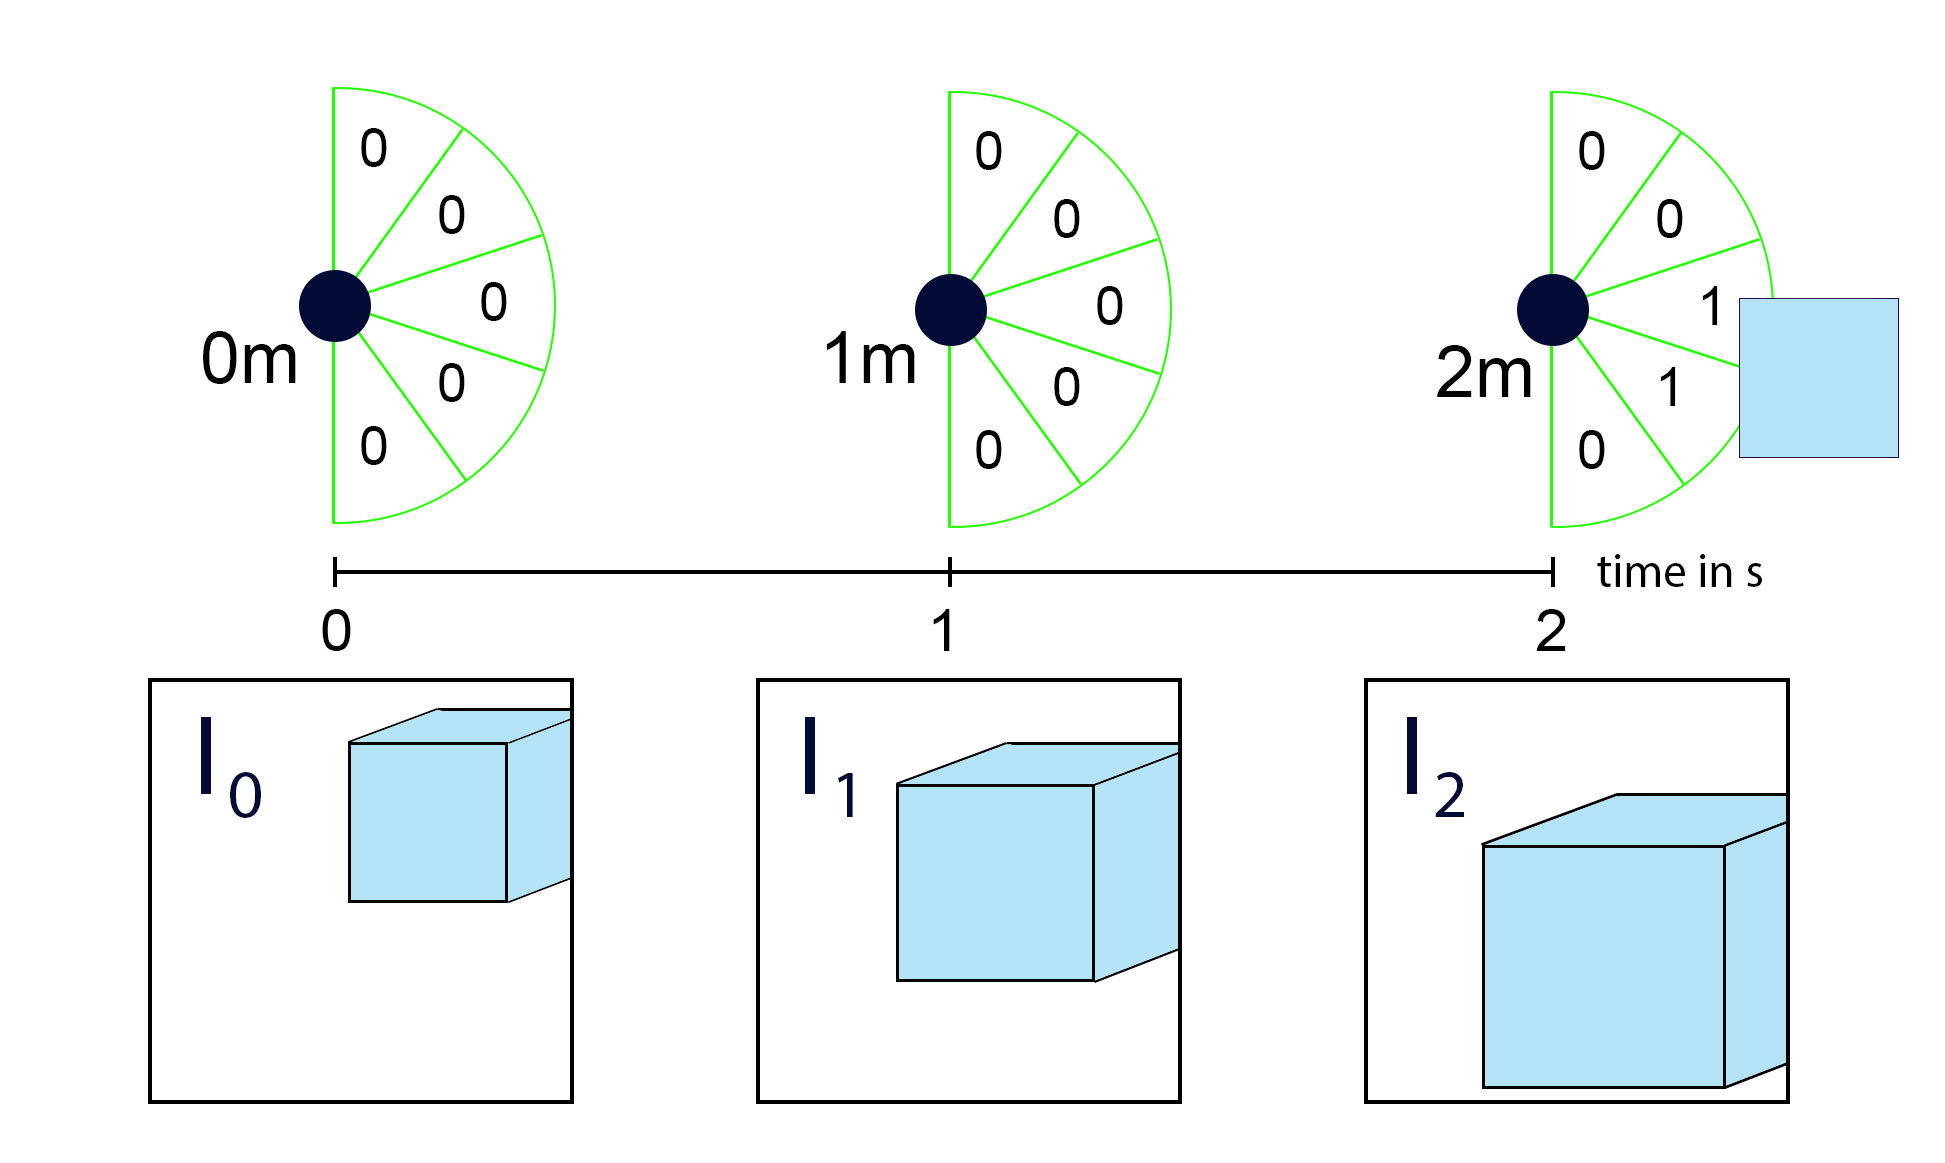
\includegraphics[width=0.75\linewidth]{Bilder/Relate_data.png} 
\caption{Concept of how images at time $t_{0}$ can be related to future laser input, if recording is taking place on a straight line. The obstacle entities are the same, but the image representations are getting larger.}
\label{relate_data}
\end{figure}

\textbf{Feature Extraction:} This step is about the autonomous creation of a dataset. The challenge is to relate images recorded at a specific time t to future laser input. The laser input is provided by a laser scanner, which returns information about recorded distances of obstacles in its vicinity. To simplify the laser input, laser distances are transferred to binary labels. To obtain binary labels for training, laser elements, need to be divided in up to n ranges, and distances to binary values if they are smaller than a specific threshold. To provide a more robust and reliable dataset, images recorded at time $t_{0}$ are not just related to laser input at time $t_{0}$, but also to laser information at future times. The concept of this can be seen at \figref{relate_data} and its corresponding table at \figref{dataset_table}, where each camera input is related to current and future laser input.

\begin{figure}[h]%[htbp]
\centering
\captionsetup{width=.75\linewidth}
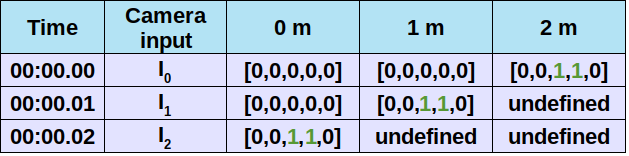
\includegraphics[width=0.75\linewidth]{Bilder/dataset_table.png} 
\caption{Finished dataset table relating images with future laser data.}
\label{dataset_table}
\end{figure}

\textbf{Training Environment:} This part is about the training of a Neural Network. As the dataset provides image data as input, the pipeline's training stage uses a Convolutional Neural Network. The entire pipeline but especially this part, is expected to be used iteratively to increase the performance of a trained model by adjusting the network's parameters.\\

\textbf{Testing:} The testing stage is about the implementation of performance metrics, to gain information about which parameters require modifications. This stage includes different types of scenarios, like the calculation of the Area under the Curve, the Analysis of a Simulated Prototype, or Visualized Models. These scenarios are highly critical to get an insight into the model's performance or hints of where to adapt, change, or replace parameters or functions.\\

\textbf{Performance Monitoring:}
At this stage of the pipeline, testing results from all previous stages are analyzed, interpreted, and documented. It further administrates all files created, continuously checks the pipeline for consistency, or tries to recognize bottlenecks or other errors, which cause the pipeline to slow down or fail. This stage is crucial, as based upon the insights given, the practitioner can decide where to change, add or adjust functions or parameters.\\

\textbf{Obstacle Avoidance Controller:} Once the model is trained, tested, and ready for deployment, it will be served as the core of an obstacle avoidance controller, which provides the model with new input data and expects it to predict reliable output about obstacles around the robot's vicinity. It is important to note that camera input alone will serve as input. At this final stage, no laser information is used.

\section{Related Work \label{RelatedWork} }
As mentioned above, self-supervised learning is about creating a supervisory signal to learn representations of data automatically or automatically create labels for a dataset. This chapter refers to projects related to self-supervised learning and provides detailed information about papers that cover robotics.\\

Self-supervised learning is used in many different fields of machine learning, like Representation Learning \cite{lee2020predicting,wang2020selfsupervised},Reeinforcement Learning \cite{xin2020selfsupervised}, Natural Language Processing \cite{meng2019selfsupervised}, Neural Networks \cite{wang2020selfsupervised,kundu2020appearance,harley2020tracking,luo2020exploring}, Generative Adversarial Networks \cite{mahapatra2020structure} and Robotics \cite{vibrationBasedLearning,nava2019learning,5979661,roboOverhead,Dahlkamp-RSS-06,932633,godard2018digging,hecke2016persistent,g2017learning} which this project is related to. \\

\cite{nava2019learning} provides the most similar concepts to this Bachelor thesis. The paper describes how to use short-range bumpers and relate them to long-range input, like images from a camera. The implementation presents a self-made robot \cite{mightyThymio}, designed for University-level educational purposes. The paper also presents a simulated performance with a Pioneer 3-AT platform in Gazebo, equipped with three cameras and a short-range sensor observing the floor's color below the robot.\\

\cite{5979661} presents an obstacle detection mechanism for humanoid navigation. The paper states that solely relying on laser range data can be problematic. The humanoid robot's sensors are located on the head, unable to recognize obstacles right in front of it. Their solution is to complement a monocular vision, located on the robot's head, with a 3-dimensional laser to create traversability labels. The paper concludes that better and more efficient navigation, a broader field of view, reduced travel time, and better performance in dealing with changes in the scene, is possible. As limitations, the authors claim, that moving obstacles or obstacles with a similar floor color can be problematic.\\

\cite{Dahlkamp-RSS-06} is also about an obstacle avoidance controller that uses a laser and a camera system as an additional long-range sensor. The implementation was presented in 2005, leading to the DARPA Grand Challenge win, a competition for autonomous vehicles, funded by the Defense Advanced Research Projects Agency. This project aimed to detect drivable surfaces in desert terrain, which is even more challenging than highways or paved roads in urban areas. The paper describes a novel algorithm that can adapt itself to different terrain types based on a self-supervised mechanism. Camera images are related to a short-range laser, responsible for scanning the vehicle's vicinity. A vision algorithm then creates a drivability map for up to 70 meters.\\

\cite{hecke2016persistent} proposes a self-supervised implementation from stereo to the monocular vision for obstacle avoidance. Their goal is to have a drone safely maneuver in a 5 X 5 m room to avoid obstacles. As a complementary sensor to monocular vision, the paper proposes a stereo-based distance estimation. This project's main challenges are to gather sufficient data for training and provide high performance in unknown environments. The article further compares its self-supervised approach to reinforcement learning, learning from demonstration, supervised learning and, unsupervised learning approaches.\\

\cite{godard2018digging} is about self-supervised monocular depth estimation. The authors provide a method that aims to create depth maps with a relatively simple model, comparing them to other self-supervised implementations, which deal with similar goals. The paper claims the results to be state-of-the-art with three main contributions introduced. Minimizing the reprojection loss corresponding to image distances between a projected and a measured point, an auto-masking loss to ignore confusion, and a multi-scale sampling method. The paper proposes that its contributions, in combination, provide an efficient model for depth estimation, trained with monocular video data, stereo data, or both combined.\\

\cite{vibrationBasedLearning} proposes a self-supervised implementation for planetary rovers. Their classification approach is about learning the visual appearance of terrain by relying on vibration-based sensing of wheel-terrain interaction. The goal is to recognize regular obstacles like rocks and cliffs and non-geometric hazards like loose sand, for example. The paper demonstrates that the self-supervised classifier should be preferred over manually trained classifiers, especially if the environment's illumination change would be faster than the manual classifier's retraining. The general performance in comparison against manual classifiers, which work on outdoor Mars-analog data sets, was shown to be as nearly as good.\\

\cite{roboOverhead} presents an implementation, including overhead imagery, to increase performance for uncrewed ground vehicles to allow them to traverse varied terrains safely. The authors claim that sensor data is often challenging to wildly take advantage of when generalizing to new environments and conditions. Overhead information is solving many problems related to autonomous robots for even the most challenging terrains due to the paper. The challenge is to properly interpret overhead data and correctly calibrate them with on-board predictions of the landscape. Similar as in the previously mentioned papers, this paper also uses several data sources and additionally self-supervised online learning to achieve a powerful long-range navigation mechanism.\\

\cite{g2017learning} describes a self-supervised technique for an unmanned aerial vehicle obstacle avoidance algorithm. The core of this approach is to combine a crash dataset in conjunction with positive data to learn a policy for navigation. The authors claim that simulation very often cannot properly transfer to real-world environments and therefore avoid it at all. The results of this project show that their implementation is effectively navigating even in cluttered environments with dynamic obstacles. The paper proposes a standard deep network architecture to train the datasets mentioned above. The article furthermore claims to outperform depth prediction based methods in several environments.
\section{Implementation \label{Implementation} }
The following chapters describe the implementation of this project in more detail. In \secref{DataAcquisition}, a Data Acquisition controller is proposed, which avoids obstacles with a laser scanner's help and saves sensor recordings as bagfiles for further processing. In \secref{FeatureExtraction}, the outputs from Data Acquisition are processed to obtain a proper dataset for training. This stage of the pipeline is called Feature extraction. Images recorded are related to laser input, where the latter serves as the necessary ground truth signal. In \secref{Training}, the training architecture and \secref{monitoring}, techniques to test, monitor, interpret and organize the results are being discussed. The training part is essential to increase performance by adjusting or replacing functions and hyperparameters. \secref{o_a_controller} proposes the implementation of some obstacle avoidance algorithms, which take as input the fully trained and developed model.\\

\figref{pipeline} displays the pipeline and its corresponding outputs.\\

\begin{figure}[h]%[htbp]
\centering
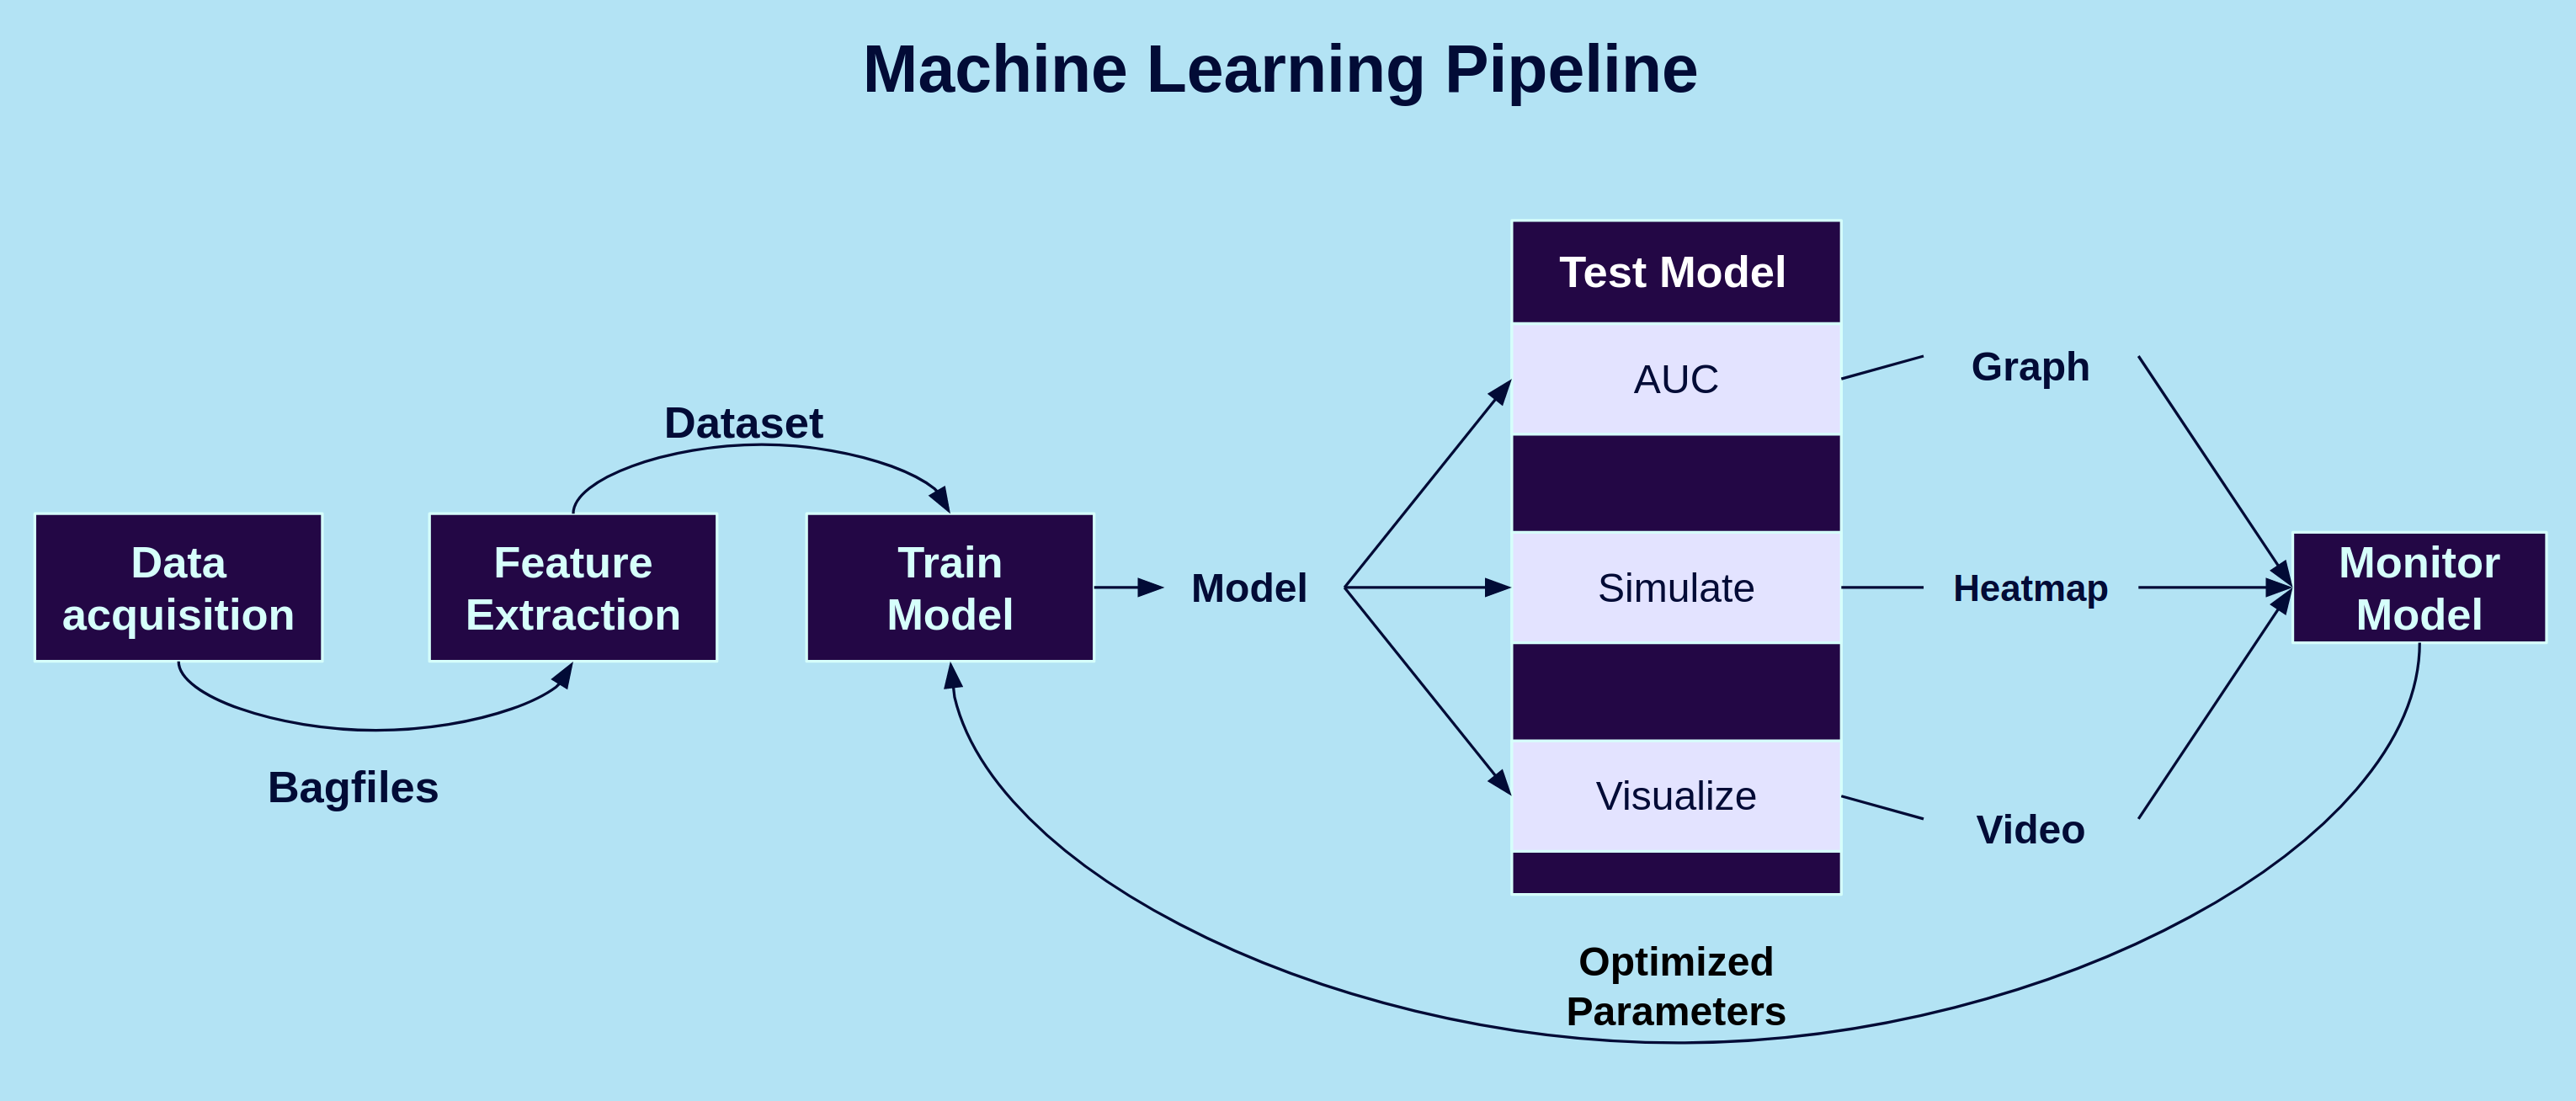
\includegraphics[width=1\textwidth]{Bilder/pipeline.png} 
\caption[]{Pipeline}
\label{pipeline}
\end{figure}
\newpage


\subsection{Data Acquisition \label{DataAcquisition} }
This chapter is about the development of a Data Acquisition
Controller, which can collect necessary data for training.\\

\subsubsection{Framework \label{framework} }
The following list provides some more details about the framework used at this step:
\begin{itemize}
\item Framework: ROS melodic
\item Simulation: Gazebo 9.0.0
\item Robot Model: TIAGo
\item PaaS: Docker 19.03.12
\end{itemize}

\subsubsection{Sensor Data \label{sensordata} }
Data acquisition records the following three sensors to provide the required data for training:
\begin{itemize}
\item Odometry
\item Laser
\item Camera
\end{itemize}

\subsubsection{Concept \label{Concept} }
As proposed in \cite{nava2019learning}, it is not efficient to have the robot randomly maneuver an environment while recording all of the sensors mentioned above. To achieve better results and prevent unnecessary recording, the controller applies a set of specifications where obstacles are actively looked for to start the recording. The recording itself is taking place while the robot is moving towards an obstacle in a straight line. \figref{straight_line} as well as \secref{FeatureExtraction} further describe this concept.\\

\begin{wrapfigure}{r}{0.45\textwidth}
\centering
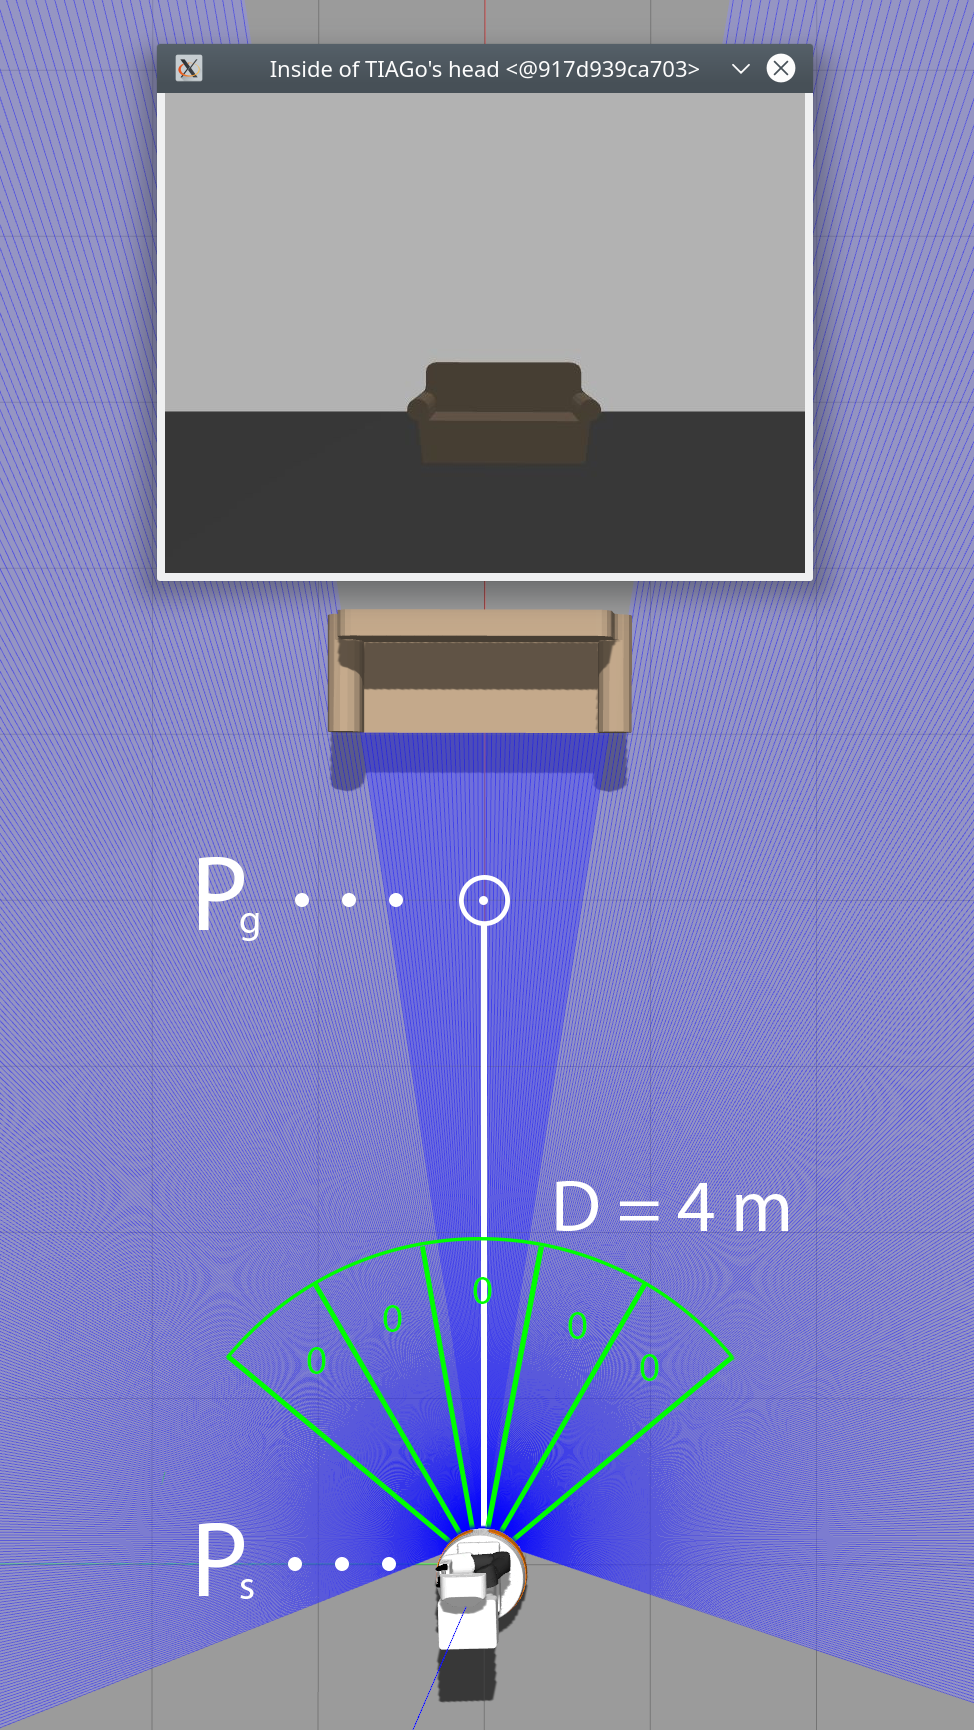
\includegraphics[width=0.35\textwidth]{Bilder/Straight_line.png}
\captionsetup{width=0.35\textwidth}
\caption{Images are related to current and also future laser input by having the robot record data and move towards an obstacle in a straight line.}
\label{straight_line}
\end{wrapfigure}
\newpage


\subsubsection{Notation \label{notation} }
The following notations describe a set of conditions that need to be met to gather data efficiently and avoid a collision while recording.\\

Let $ P_{s} $ be a coordinate from where the recording starts and $ P_{g} $ a
coordinate where the recording ends and let the shortest distance between $ P_{s} $ and $ P_{g} $ be $ D $, the trajectory on where the recording is taking place. The robots own position is noted as $ P_{r} $ and let the Laser at the robots longitudinal axis be $ L_{0} $. To define a safe passage towards an obstacle, it is further necessary to define $ D_{s} = D_{r} + r $ where $ D_{r} $ stands for the robots diameter and $ r $ for a constant, big enough to avoid collisions.\\

The distance $ D $ is a flexible parameter and can be adjusted among different models trained, but has to be kept consistent for each pipeline run.\\

To obtain possible coordinates for $ P_{s} $ and $P_{g}$, and to guarantee a safe passage towards the obstacle, following conditions have to be met

\begin{equation}
\label{eqn:1}
F = \{P_{s} |L_{0} - safe_{d} - D = P_{s} \mbox{~and~} P_{s} > 0\} 
\end{equation}

\begin{equation}
\label{eqn:2} 
F = \{P_{g} |L_{0} - safe_{d} = P_{g} \mbox{~and~} P_{g} + safe_{d} > D \}  
\end{equation}

\begin{equation}
\label{eqn:3} 
F = \{D_{s} |\frac{D_{s}}{2} < \sin(\alpha) * L_{0->n}\}  
\end{equation}

where $ safe_{d} $ stands for a safe distance
from $ P_{g} $ to the obstacle, the robot
is not supposed to cross, and $ L_{0->n} $ stands for all Lasers available on the robot. To increase performance, $ L_{0->n} $ can also be limited to a specific range around $ L_{0} $, to decrease calculations necessary at this step. \figref{safe_passage} shows the safe passage concept in more detail, where all conditions for a safe passage are met at the left, and some conditions are not met at the right image.

\begin{figure}[H]%[htbp]
\centering
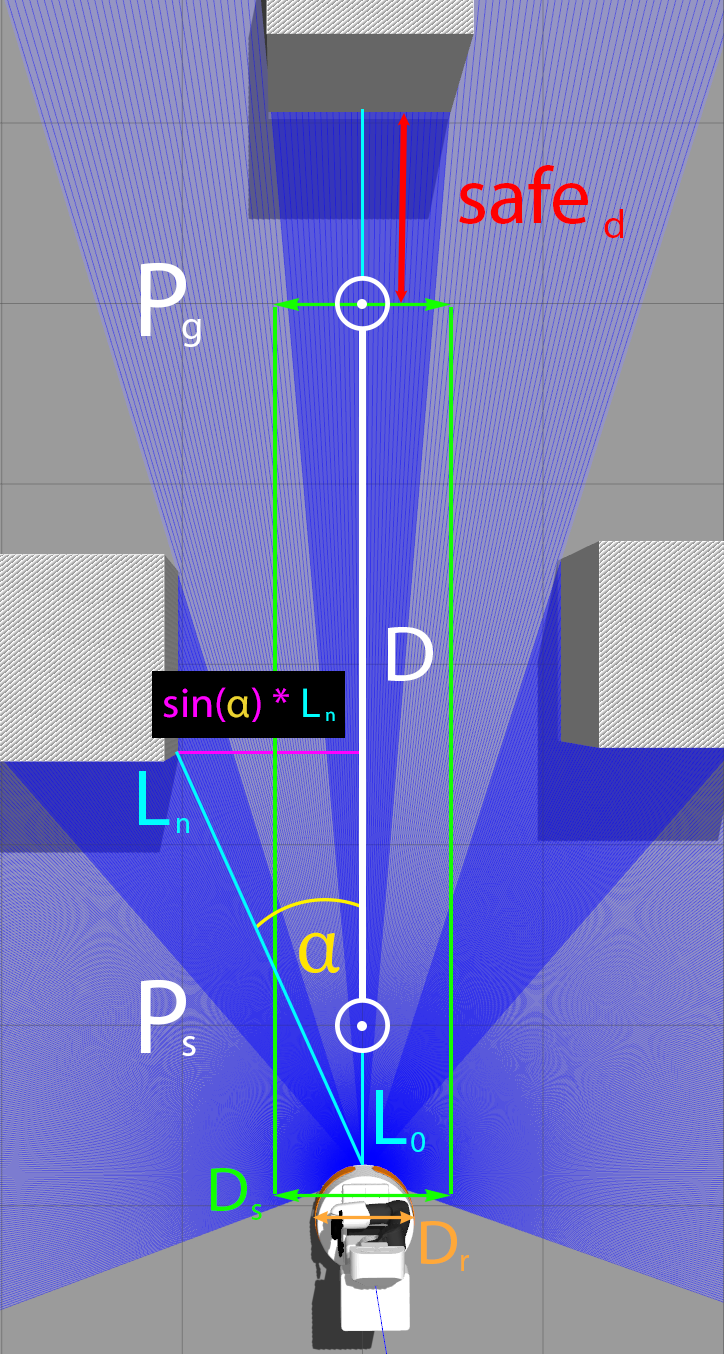
\includegraphics[width=0.30\textwidth]{Bilder/Safe_passage_true_final.png} 
\hspace{1.0 cm}
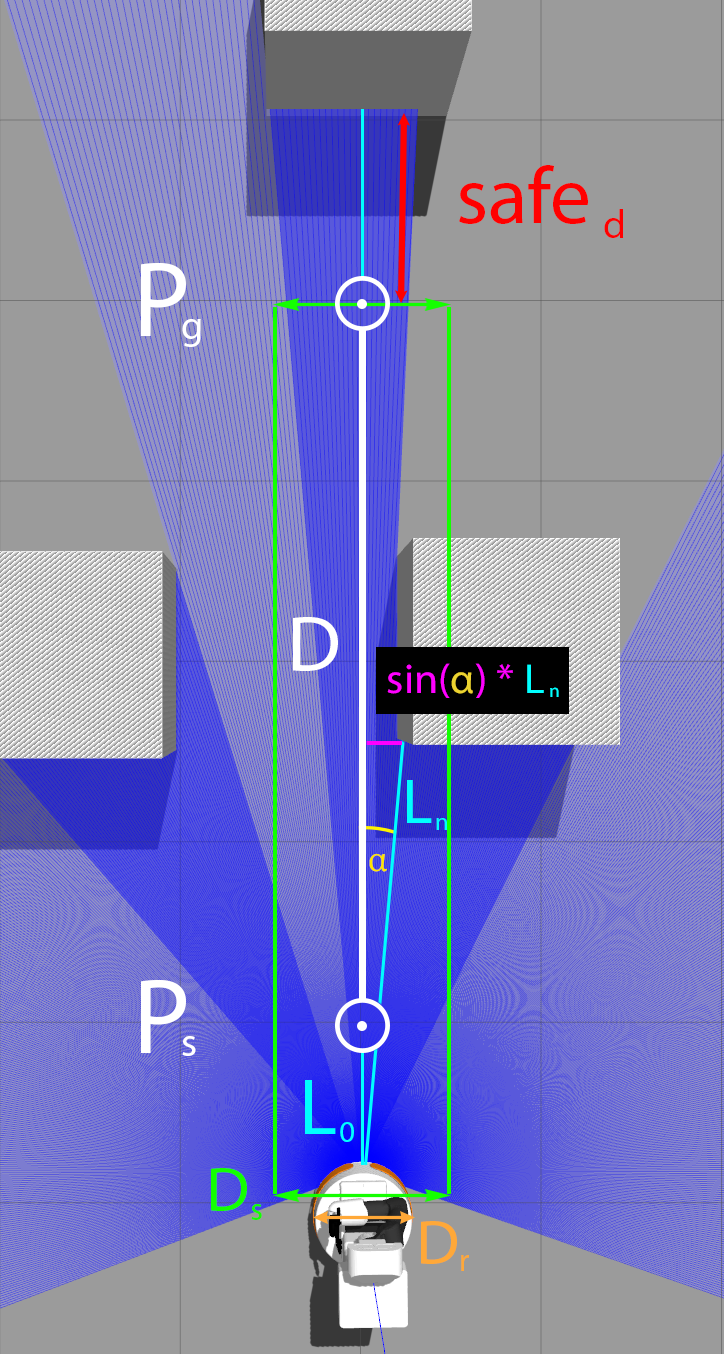
\includegraphics[width=0.30\textwidth]{Bilder/Safe_passage_false_final.png} 
\caption[]{Concept of the conditions required to guarantee a safe passage from $ P_{s} $ to $ P_{g} $. While the left image shows an example of the safe zone to be free, depicted as the area between the two green lines with a diameter of $ D_{s} $, the right image's safe zone intersects with an obstacle. Therefore, $ P_{g} $ at the right image would not be a valid candidate for recording.}
\label{safe_passage}
\end{figure}

\subsubsection{State Machine \label{state_machine} }
The algorithm is set up as a state machine to provide a fully autonomous gathering and saving of data while avoiding obstacles. Each state completes a well-defined task to efficiently cover all steps or substeps needed. \figref{statemachine} displays all defined states.

\begin{figure}[H]%[htbp]
\centering
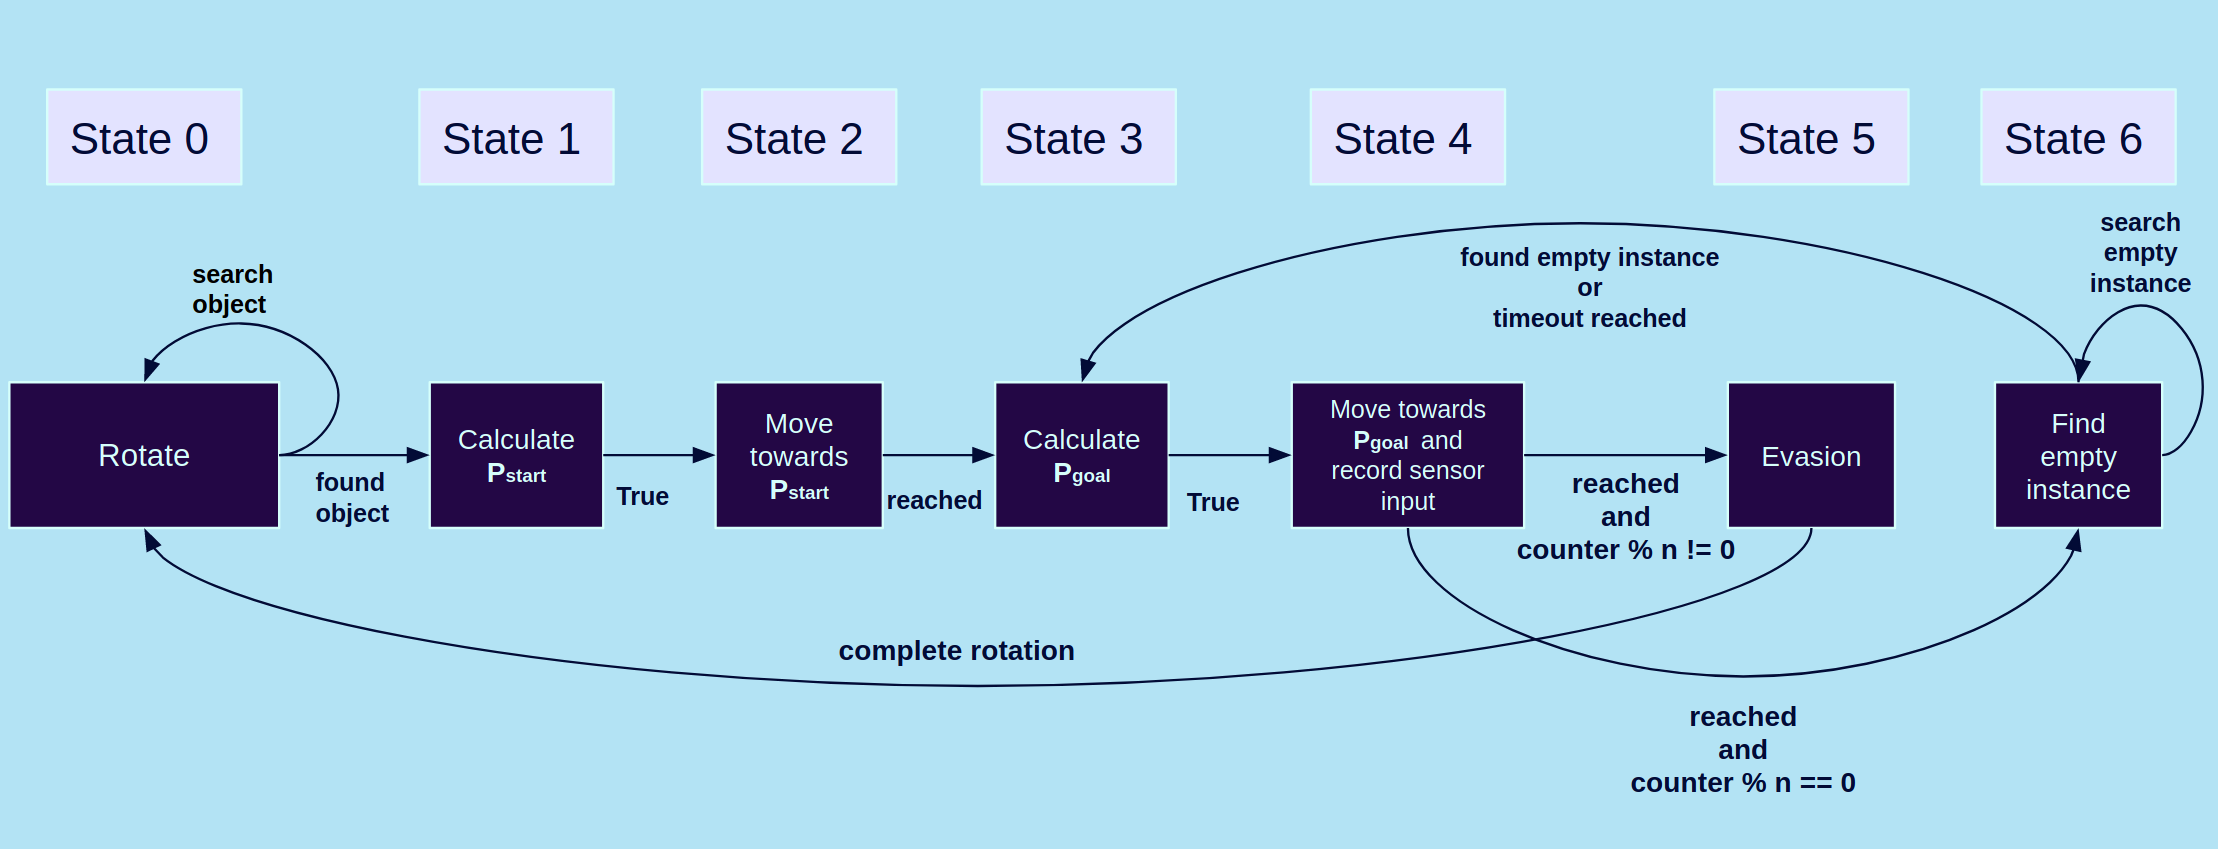
\includegraphics[width=1\textwidth]{Bilder/StateMachineChart.png} 
\caption[]{State Machine}
\label{statemachine}
\end{figure}

\newpage

\textbf{State 0}\\
This state is the initial state after launching the robot. The robot will immediately start to rotate and try to find a goal $ P_{g} $, while observing defined conditions \ref{eqn:1}, \ref{eqn:2} and \ref{eqn:3}. Once the algorithm finds a possible candidate with all conditions met, the robot's state is transitioned to 1.\\

\textbf{State 1}\\
At this state, the robot is calculating $ P_{s} $, which stands for the
starting position of the recording. To provide the proper coordinates to the robot's navigation, $ P_{s} $ needs to be transferred from robot to world coordinates. The calculation can be done as
\begin{equation}
\label{eqn:4} 
\vec{P}_{s_{world}}=
\vec{P}_{s}*
  \begin{bmatrix}
    \cos(\alpha) & -\sin(\alpha)\\
    \sin(\alpha) & \cos(\alpha)
  \end{bmatrix}+
\vec{P}_{r_{world}}
\end{equation}

where $ P_{r_{world}} $ stands for the robot's position in world coordinates and $ P_{s_{world}} $ for the starting position, which can be directly fed to the robot's motion sensors. Once the calculation is done, the outputs calculated are given to the next state.\\

\textbf{State 2}\\
At this state, the robot is just moving towards the starting position. Once a specific threshold around $ P_{s} $ is reached, the robot's state is transitioned to 3.\\

\textbf{State 3}\\
Here, the robot's location is exactly on top of the starting position, focusing on the obstacle. The goal coordinates $ P_{g} = L_{0} - safe_{d} $ are multiplied with the  transformation matrix defined at \ref{eqn:4}, to obtain $ P_{g_{world}}$, which can also be given directly to the motion sensors of the robot. Once the calculation is done, the coordinates calculated are given to state 4.\\

\textbf{State 4}\\
Like state 2, the robot will move towards the goal given, which is $ P_{g} $. It is important to note that during state 4, the recording of sensor data is taking place. Once $ P_{g} $ is reached, the recordings are saved, and the robots state is transitioned to 5.\\

\textbf{State 5}\\
At this state, the robot, will randomly either turn to the right or the left, to prevent getting caught in a loop, or accidentally collide with objects close by. The angle to rotate away from the obstacles, is flexible and can be set as a parameter. The value can also be randomized to provide a higher degree of recording variety. Once the robot has turned away from the obstacle, the state is set back to 0.\\  

Even though a rotation for a specific angle sounds trivial, the robot can easily overshoot and get stuck in a flipping state with insanely large inputs given to the angle motion control. This is caused by $\theta$, which displays the robot's angle orientation, for the first and second quadrant defined from $ 0 $ to $ \pi $, and for the third and fourth quadrant from $-\pi$ to $ 0 $. To prevent flipping, $\theta$ can be mapped to

\begin{equation}
\label{eqn:5} 
\theta_{alt}(\theta) =
\begin{cases}
2\pi + \theta, &\{\theta |-\pi\leq \theta \leq 0 \}\\
\theta,			&{otherwise}
\end{cases}
\end{equation}

to a range from $ 0 $ to $2\pi$. This has the advantage that just one flip instead of $ 2 $ need to be observed. A flip in this context means a sudden change of sensor inputs like from $\pi$ to $-\pi$, for example. The left image of \figref{theta_alt} shows the mapping from $\theta$ to $\theta_{alt}$. A turn from $\frac{\pi}{2}$ to $\pi$, for example, is rather simple and can be generally achieved with

\begin{equation}
\label{eqn:6} 
f(\theta_{alt}) = \theta_{goal} - \theta_{alt}
\end{equation}

This function can just be applied if the required rotation is not bigger than $2\pi-\theta_{start}$. If a turn in a clockwise direction of $ 180 $ degrees or in radian $\pi$ is required, where $\theta_{start}$ has the value of $\frac{3\pi}{2}$ for example, $\theta_{goal}$ can be considered as $\frac{\pi}{2}$ or better $\frac{5\pi}{2}$. The latter allows equation \ref{eqn:6} to be applied with some minor changes as follows:\\

\begin{equation}
\label{eqn:7} 
f(\theta_{alt}) =
\begin{cases}
\theta_{goal} - \theta_{alt}, &\{\theta_{alt} |\theta_{start} \leq \theta_{alt} \leq 2\pi \}\\
\theta_{goal} - (2\pi + \theta_{alt}), &{otherwise}
\end{cases}
\end{equation}

This case can be seen at the right image of \figref{theta_alt} where the upper case of the equation \ref{eqn:7} applies from $\theta_{start}$ to $2\pi$ and the lower case from $0$ to $\theta_{goal}$.\\

\textbf{State 6}\\
State 6 is just triggered every $ n $ recordings. It is attempted to search an area without obstacles and record an instance with images solely displaying the empty floor and sky. This state is necessary to have the prediction classifying images without barriers accordingly. Once a blank area is found, the robot's state will be transitioned to 3, to have the robot moving forward from its current position while recording sensor input. The forward distance to cover is the same as defined at \secref{notation}. If the robot cannot find any empty area for a period of $ n $ seconds, the state is set to $ 0 $ to avoid the robot getting stuck in a loop. This can happen in very dense environments where many obstacles surrounding the robot.\\

\begin{figure}[h]%[htbp]
\centering
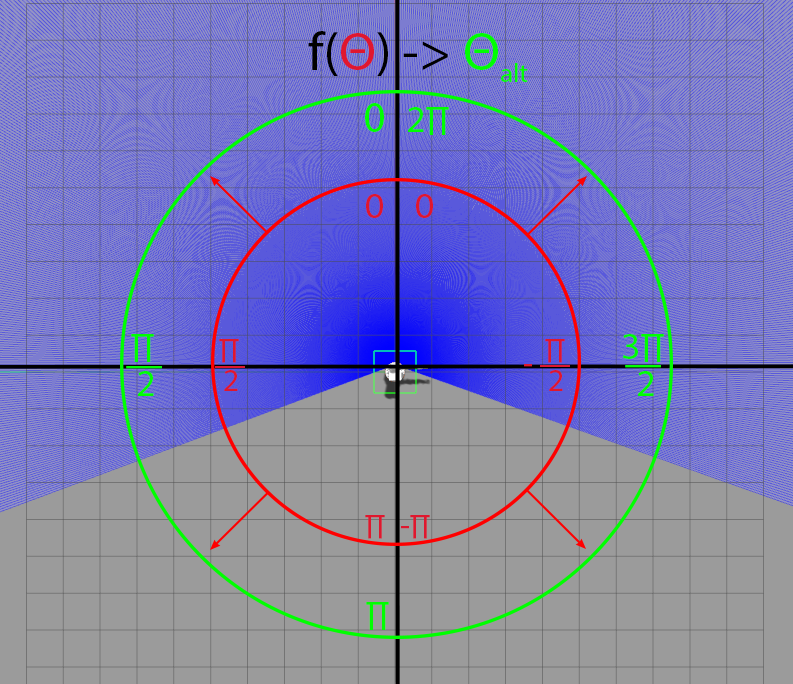
\includegraphics[width=0.45\textwidth]{Bilder/theta_thetaAlt.png} 
\hspace{0.3 cm}
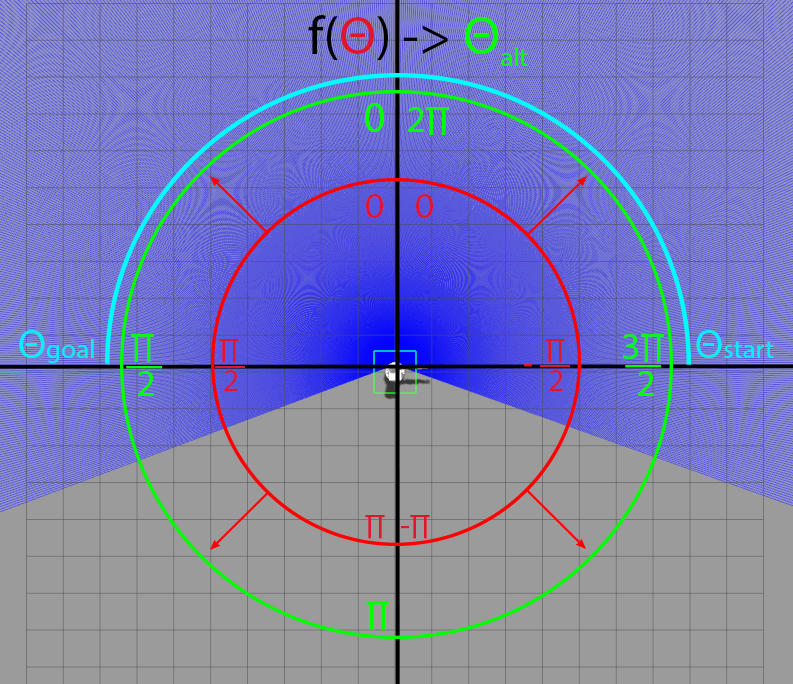
\includegraphics[width=0.45\textwidth]{Bilder/theta_thetaAlt_example.png} 
\caption[]{The left figure shows the mapping from $\theta$ to $\theta_{alt}$ while the right figure shows a rotation of 180 degree from $\theta_{start}$ to $\theta_{goal}$.}
\label{theta_alt}
\end{figure}

\subsubsection{Bagfiles \label{bagfiles} }
Once the robot reaches the number of bagfiles he is required to record, the program will automatically stop and copy all recorded files to a folder, marking the folder and files with an index to make them recognizable for a specific pipeline run.  It is important not to copy unfinished bagfiles, as this can cause subsequent stages to fail.  The node implements a mechanism which prevents to use incomplete files. At further stages, once bagfiles are opened, they are additionally checked for consistency or duplicates, as this can also cause the pipeline to fail. For a recording distance of approximately three meters, each bagfile contains about 60 instances of sensor input with odometry, laser, and image information.
\newpage

\subsection{Feature Extraction \label{FeatureExtraction} }

\begin{wrapfigure}{r}{0.45\textwidth}
\centering
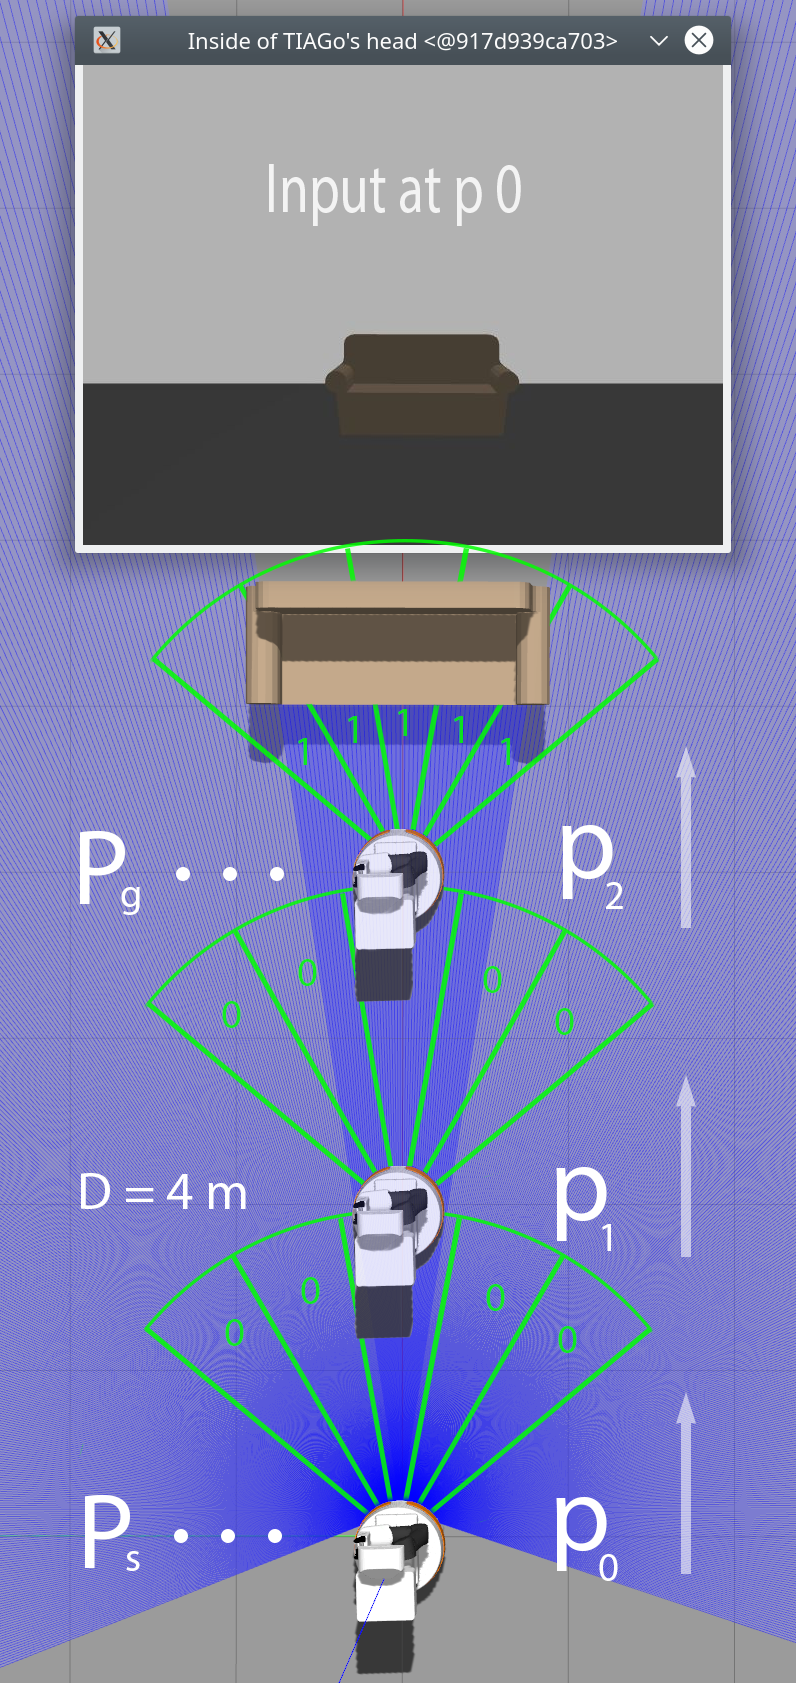
\includegraphics[width=0.35\textwidth]{Bilder/FeatureExtraction_5.png}
\captionsetup{width=0.35\textwidth}
\caption{Simplified concept of how to relate camera input at $p_{0}$ to subsequent positions of laser input.}
\label{featureExtraction5}
\end{wrapfigure}

This chapter describes how bagfiles are processed to create an h5py dataset for training as the second stage of this pipeline. The main goal at this step is to properly relate all recorded sensor input in an efficient self-supervised manner. As a general concept, the ideas proposed by \cite{nava2019learning} are applied to extract all necessary information from the recorded sensor data. \cite{nava2019learning} as well as \cite{5979661} or \cite{Dahlkamp-RSS-06} all suggest a laser or a bumper, to provide supervisory signals, which can be used as the corresponding ground truth for camera input. The easiest way to relate camera input and laser data is to relate inputs recorded simultaneously. After training a model on such a dataset, it could be used to predict a distance for every camera input. While this concept can provide already some efficient prediction, \cite{nava2019learning} describes how to relate camera input at time $t$, not just to bumper input at time $t$, but also to bumper input at time $t_{0 -> n}$. This is possible if the recording is taking place on a straight line, as depicted in \figref{straight_line}.\\

If the set of $\{p_{0},...,p_{n}\}$, are all intermediary positions covered from $P_{s}$ to $P_{g}$, an input image recorded at one of these positions, can be related to any subsequent supervisory data, up to $P_{g}$. \figref{featureExtraction5} shows a simplified example about this concept, where an image as input at $p_{0}$, is related to supervisory data from $p_{0}$ up to $p_{2}$. The following table shows this simplified example as a dataset for one single instance. $p_{2}$ in this example would be $P_{g}$ and therefore the end of the recording. \\

%\begin{table}[h]
%\resizebox{\columnwidth}{!}{%
%\begin{tabular}{|
%>{\columncolor[HTML]{FFFFFF}}l |
%>{\columncolor[HTML]{FFFFFF}}l |
%>{\columncolor[HTML]{DAE8FC}}l |
%>{\columncolor[HTML]{DAE8FC}}l |
%>{\columncolor[HTML]{DAE8FC}}l |
%>{\columncolor[HTML]{DAE8FC}}l |
%>{\columncolor[HTML]{DAE8FC}}l |
%>{\columncolor[HTML]{ECF4FF}}l |
%>{\columncolor[HTML]{ECF4FF}}l |
%>{\columncolor[HTML]{ECF4FF}}l |
%>{\columncolor[HTML]{ECF4FF}}l |
%>{\columncolor[HTML]{ECF4FF}}l |
%>{\columncolor[HTML]{DAE8FC}}l |
%>{\columncolor[HTML]{DAE8FC}}l |
%>{\columncolor[HTML]{DAE8FC}}l |
%>{\columncolor[HTML]{DAE8FC}}l |
%>{\columncolor[HTML]{DAE8FC}}l |}
%\hline
%{\color[HTML]{000000} }              & {\color[HTML]{000000} }                      & \multicolumn{5}{c|}{\cellcolor[HTML]{6665CD}{\color[HTML]{FFFFFF} \textbf{$p_{0}$}}}                                                                                                                            & \multicolumn{5}{c|}{\cellcolor[HTML]{9698ED}{\color[HTML]{FFFFFF} \textbf{$p_{1}$}}}                                                                                                                            & \multicolumn{5}{c|}{\cellcolor[HTML]{6665CD}{\color[HTML]{FFFFFF} \textbf{$p_{2}$}}}                                                                                                                            \\ \hline
%{\color[HTML]{000000} \textbf{Time}} & {\color[HTML]{000000} \textbf{Camera input}} & {\color[HTML]{000000} \textbf{$R_{1}$}} & {\color[HTML]{000000} \textbf{$R_{2}$}} & {\color[HTML]{000000} \textbf{$R_{3}$}} & {\color[HTML]{000000} \textbf{$R_{4}$}} & {\color[HTML]{000000} \textbf{$R_{5}$}} & {\color[HTML]{000000} \textbf{$R_{1}$}} & {\color[HTML]{000000} \textbf{$R_{2}$}} & {\color[HTML]{000000} \textbf{$R_{3}$}} & {\color[HTML]{000000} \textbf{$R_{4}$}} & {\color[HTML]{000000} \textbf{$R_{5}$}} & {\color[HTML]{000000} \textbf{$R_{1}$}} & {\color[HTML]{000000} \textbf{$R_{2}$}} & {\color[HTML]{000000} \textbf{$R_{3}$}} & {\color[HTML]{000000} \textbf{$R_{4}$}} & {\color[HTML]{000000} \textbf{$R_{5}$}} \\ \hline
%{\color[HTML]{000000} 00:00:01}      & {\color[HTML]{000000} {[}178, ... , 255{]}}  & {\color[HTML]{000000} 0}                & {\color[HTML]{000000} 0}                & {\color[HTML]{000000} 0}                & {\color[HTML]{000000} 0}                & {\color[HTML]{000000} 0}                & {\color[HTML]{000000} 0}                & {\color[HTML]{000000} 0}                & {\color[HTML]{000000} 0}                & {\color[HTML]{000000} 0}                & {\color[HTML]{000000} 0}                & {\color[HTML]{000000} 1}                & {\color[HTML]{000000} 1}                & {\color[HTML]{000000} 1}                & {\color[HTML]{000000} 1}                & {\color[HTML]{000000} 1}                \\ \hline
%\end{tabular}
%}
%\caption{Simplified dataset output}
%\label{tab:example_prediction}
%\end{table}



\begin{table}[h]
\resizebox{\columnwidth}{!}{%
\begin{tabular}{|c|c|
>{\columncolor[HTML]{D6FFFB}}c |
>{\columncolor[HTML]{D6FFFB}}c |
>{\columncolor[HTML]{D6FFFB}}c |
>{\columncolor[HTML]{D6FFFB}}c |
>{\columncolor[HTML]{D6FFFB}}c |
>{\columncolor[HTML]{B3E3F4}}c |
>{\columncolor[HTML]{B3E3F4}}c |
>{\columncolor[HTML]{B3E3F4}}c |
>{\columncolor[HTML]{B3E3F4}}c |
>{\columncolor[HTML]{B3E3F4}}c |
>{\columncolor[HTML]{D6FFFB}}c |
>{\columncolor[HTML]{D6FFFB}}c |
>{\columncolor[HTML]{D6FFFB}}c |
>{\columncolor[HTML]{D6FFFB}}c |
>{\columncolor[HTML]{D6FFFB}}c |}
\hline
\multicolumn{1}{|l|}{} & \multicolumn{1}{l|}{} & \multicolumn{5}{c|}{\cellcolor[HTML]{020B36}{\color[HTML]{FFFFFF} $p_{0}$}} & \multicolumn{5}{c|}{\cellcolor[HTML]{020B36}{\color[HTML]{FFFFFF} $p_{1}$}} & \multicolumn{5}{c|}{\cellcolor[HTML]{020B36}{\color[HTML]{FFFFFF} $p_{2}$}} \\ \hline
\textbf{Time}          & \textbf{Camera Input} & $R_{1}$       & $R_{2}$       & $R_{3}$       & $R_{4}$      & $R_{5}$      & $R_{1}$       & $R_{2}$       & $R_{3}$       & $R_{4}$      & $R_{5}$      & $R_{1}$       & $R_{2}$       & $R_{3}$       & $R_{4}$      & $R_{5}$      \\ \hline
00:00:01               & {[}178,...256{]}      & 0             & 0             & 0             & 0            & 0            & 0             & 0             & 0             & 0            & 0            & 1             & 1             & 1             & 1            & 1            \\ \hline
\end{tabular}
}
\caption{Simplified dataset output}
\label{tab:example_prediction}
\end{table}



\subsubsection{Finding positions on a simplified example \label{finding_positions} }
The amount of intermediary positions of the set $\{p_{0},...,p_{n}\}$ is flexible. It makes sense to distribute them over $D$ evenly. In \figref{straight_line}, $D$ was set to 4 meters. If the amount of 40 were chosen as intermediary positions, every input image would be related to laser data from position $p_{0}$ to $p_{39}$. Table \ref{tab:example_prediction}, in this case, would be relatively larger, as the columns would go from $\{p_{0},...,p_{39}\}$. The number of positions and $ D $ itself, should also depend on the camera and the type of supervisory signals used. It is important to note, that for each dataset, the number of positions should remain the same, which in the simplified example of \figref{featureExtraction5} would be $\{p_{0},...,p_{2}\}$. In this example, $D$ is set to 4 meters. To properly relate input data, coming from bagfiles, each position in $\{p_{0},...,p_{2}\}$ needs to get a fixed distance. As $p_{0}$ is equal to the starting position $P_{s}$, it is set to zero. $p_{1}$ would be set to 2m and $p_{2}$ to 4m, which is equal to the goal position $P_{g}$. More generally, the intermediary positions can be calculated as

\begin{equation}
\label{eqn:8} 
f(n) = n * \frac{D}{a-1}
\end{equation}

where $n$ stands for each individual position and $a$ for the amount of the set $\{p_{0},...,p_{n}\}$. Using the data of \figref{featureExtraction5}, following tuple, which will be used in the simplified example described below, can be generated as $(\{p_{0},0m\},\{p_{1},2m\},\{p_{2},4m\})$.\\

In \figref{featureExtraction5}, the amount of laser data generated over the distance of 4 meters highly exceeds the number of positions set. For every image, proper laser data, which is recorded at the exact or at a very close position of the set positions $(\{p_{0},0m\},\{p_{1},2m\},\{p_{2},4m\})$, need to be searched for. This can be achieved in 2 steps.\\ 

At first, all individual bagfiles with camera, laser, and odometry input need to be related in one coherent table, where the recording time serves as the index for each row. Images, laser data, and positional values of the robot serve as columns. An example of such a table can be seen in the left image of \figref{relative_positions}. The example table contains 40 rows of data. The goal is to reach an output similar to the table \ref{tab:example_prediction}, with just images and their respective binary ground truth labels.\\

At second, once the coherent table has been set up for all input values, every image is supposed to be related to its current and future laser values, by simply checking which distance closely corresponds to the distances of $(\{p_{0},0m\},\{p_{1},2m\},\{p_{2},4m\})$ as in the simplified example.\\

Demonstrating how to relate images with future laser data, the row with index 18 of the right image of \figref{relative_positions} can be analyzed. The goal is to relate the image data of this row to future laser input. This can be achieved by picking all subsequent rows and check, which of the subsequent rows positional values match or are closest to the distances of
$(\{p_{0},0m\},\{p_{1},2m\},\{p_{2},4m\})$. It is important to note that the index 18's positional values' perspective is considered the zero point coordinate. The positional values from all subsequent rows are set concerning the index 18 coordinate system. As the recording has been on a straight line, the positions from $(\{p_{0},0m\},\{p_{1},2m\},\{p_{2},4m\})$ can be looked up at the subsequent positional values, which are set relative to index 18. The matching ones are chosen, and their corresponding laser data is used to relate with the image of index 18. In the right example image of \figref{relative_positions}, the chosen ground truth laser data would be those of index 38.\\

In the next subsection, the transformation from actual laser distances to binary labels are discussed in more detail. This also explains why there are five subcolumns in the output table \ref{tab:example_prediction}, depicted as $R$ and no real laser distances.

\begin{figure}[h]%[htbp]
\centering
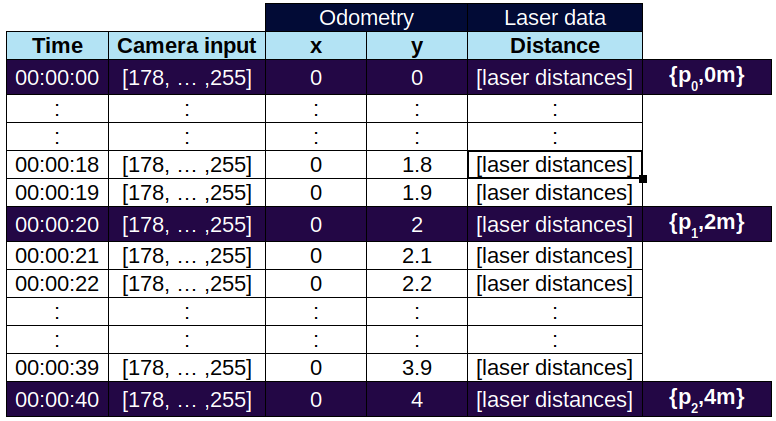
\includegraphics[width=0.48\textwidth]{Bilder/positions.png} 
\hspace{0.2 cm}
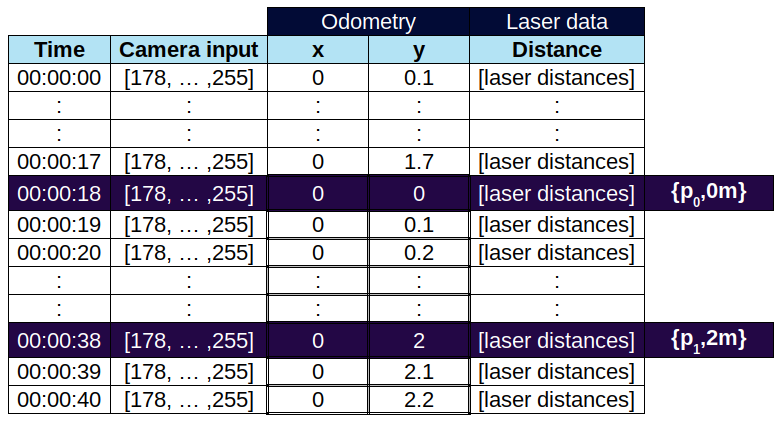
\includegraphics[width=0.48\textwidth]{Bilder/relative_positions.png} 
\caption[]{The left image shows a simplified example of bagfiles, related to one coherent table. The right image shows of how all subsequent positional values of index 18, are set relative to index 18 and how subsequently, laser data, of positions close to values from $(\{p_{0},0m\},\{p_{1},2m\},\{p_{2},4m\})$, are chosen as future ground truth labels for the image with the index 18.}
\label{relative_positions}
\end{figure}

\subsubsection{Laser distance to binary values\label{laser_binary} }
Looking at the output dataset example table \ref{tab:example_prediction}, the laser fields $\{R_{1}, ... , R_{5}\}$ for each distance of $\{p_{0},...,p_{n}\}$ do not contain distances but binary values. Those values indicate whether an obstacle was touching a specific range of set $\{R_{1}, ... , R_{5}\}$ at a specific time. Generally, it would be possible to use distances instead of binary labels, but as not just laser input at time $t$, but also laser input at time $t_{0->n}$, is related to current images, the distances of objects can be predicted rather accurate, with much less computational effort. In \figref{featureExtraction5}, the number of ranges is set to 5, and the distance threshold to about 1.8 meters. Those parameters are flexible but need to be kept static for each pipeline run.\\

Bagfiles return an extensive array of 666 distance values. Each of these values stands for one laser recorded at time t. The array then is split up in ranges, and for each range, a threshold like 

\begin{equation}
\label{eqn:9} 
f(R_{n}) =
\begin{cases}
$1$, & \forall x; x \in R_{n}; x \leq d_{threshold},\\
$0$,			&{otherwise}
\end{cases}
\end{equation}

is applied to obtain the binary output signals. At \figref{featureExtraction5} as well as in table \ref{tab:example_prediction}, the laser input at $p_{2}$ is set to $1$, as for all 5 ranges an obstacle close by is detected.

\subsubsection{Unknown labels \label{unknownLabels} }
While in the right image of \figref{relative_positions}, an intermediary position for index 18 is found, it is possible that due to odometry drift, no intermediary position can be obtained within a reasonable range. In the example, index 18 can be related to index 38 with position $p_{1}$, as index 38 is exactly 2 meters away from index 18. These exact values do not reflect realistic behavior. Therefore, a fixed range needs to be set up to define positions as valid or not. While labels with valid positions can be immediately used, labels with invalid positions are set to unknown. This behavior is one reason why \cite{nava2019learning} proposed that recording should occur while the robot moves on a straight line towards an obstacle. A side effect of the robot moving towards the obstacle on a straight line is the decreasing number of labels, where no position can be found. \secref{Training} will discuss of how unknown labels are treated with during training.
\newpage

\subsection{Training Architecture \label{Training} }
Once the dataset is finished and saved as an h5py file, it will be fed directly into a Convolutional Neural Network. The network is based on the LeNet architecture further described in \cite{726791}.\\

Table \ref{tab:example_prediction} displays an example row of how the dataset is being delivered to the CNN. As input serves the normalized image, set to the shape of (64,80,3). The output shape depends on the number of intermediary positions and on the number of laser ranges set. In the example table \ref{tab:example_prediction}, the output shape is (1,15). Due to \cite{nava2019learning}, the general learning problem is considered a multi-label binary classification with incomplete training labels, which predicts m sensor values at n intermediary positions, while being served one image as input. The incompletion of training labels derives from the fact that not all intermediary positions might be found for each camera input. In this case, labels are set to unknown. To avoid labels being set to unknown during Feature Extraction, it is important just to record data while moving on a straight line towards the obstacle, as discussed in \secref{DataAcquisition}. This measure does not completely lead to all intermediary positions found, \cite{nava2019learning} suggests using a technique implemented in \cite{DBLP:journals/corr/EigenPF14}, where a binary mask is created, which contains one value for each label. Labels are classified as $0$ if unknown and as $1$ otherwise. The mask is then multiplied during forward propagation with the error signal (prediction - ground truth), leading to unknown labels to be nullified.

\begin{figure}[h]%[htbp]
\centering
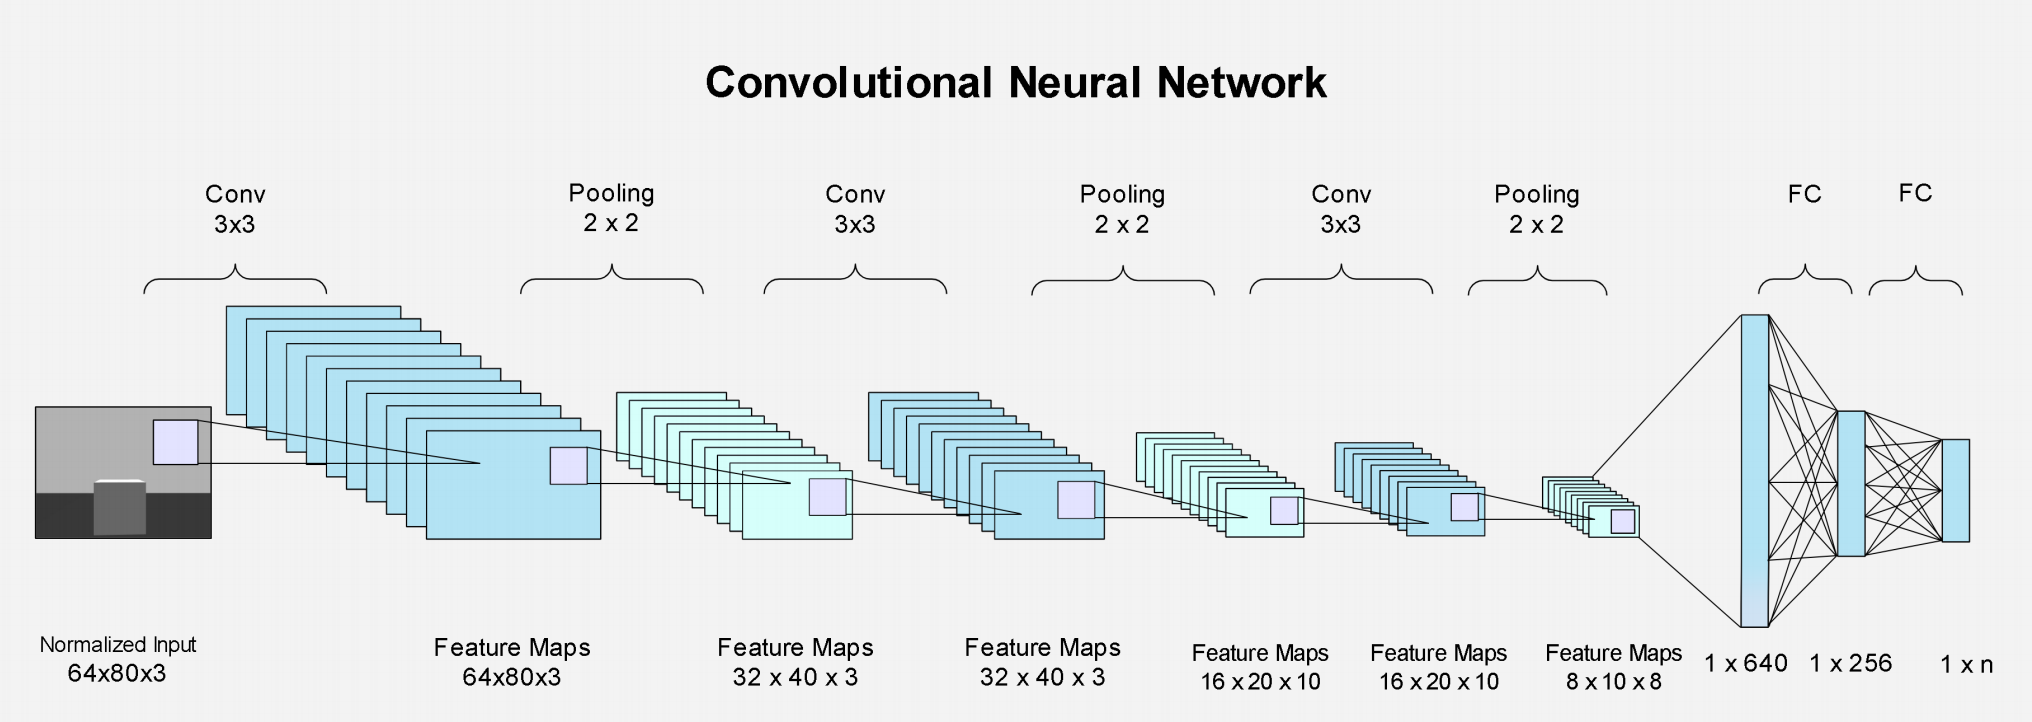
\includegraphics[width=1\textwidth]{Bilder/architecture.png} 
\caption[]{Architecture}
\label{architecture}
\end{figure}

The following list and \figref{architecture} further describe the most important features of the architecture used. Some parameters are adjustable and will be changed after the testing results had been monitored.
\begin{itemize}
\item Normalized input shape (64,80,3)
\item Output shape (1,n)
\item Epochs: 15 - 30
\item Steps per Epoch: 1000
\item Learning rate: 0.0002 - 0.0004
\item Optimizer: ADAM
\item Loss Function: mean squared
\item Batch Size: 64
\item Output: Model, Graph (training vs validation loss)
\end{itemize}

After the training is finished, the model can be used for testing, deployment, or visualization. The training part of the pipeline furthermore creates a graph that displays the validation and test loss. Several of these graphs and their interpretations are discussed in \secref{ExperimentalResults}.
\newpage

\subsection{Performance Monitoring and Testing \label{monitoring} }
At this stage, the entire pipeline is monitored and tested. The goal is to get an insight into where and what changes need to be made to increase the pipeline's performance. \cite{ Goodfellow-et-al-2016} suggests the following process about testing and monitoring:

\begin{itemize}
\item It should be clearly defined what type of error metric will be used, and which target value is tried to reach. The implementation should relate the metrics to the general goal of the application.

\item A functioning pipeline should be developed as fast as possible, including estimating the appropriate performance metrics.

\item A mechanism should be implemented to recognize bottlenecks and supervise components that are not performing as expected.

\item The pipeline should retrain the model, apply incremental changes, add new data, adjust hyperparameters, or change algorithms based on the analysis results.
\end{itemize}

The following subsections will cover performance metrics, hyperparameters, tests on a deployed simulation prototype, visualization of predictions, and a file administration class while attempting to complete the suggestion of Ian Goodfellow.

\subsubsection{Metrics \label{metrics} }
As the prediction of the model, given an image as input, is a set of probabilities and the corresponding ground truth are binary labels, \cite{nava2019learning} proposes to use the Receiver Operating Characteristics curve (ROC) and its related Area (AUC) as performance metrics for this type of implementation.\\ 

Due to \cite{rakotomamonjy2004optimizing}, the Receiver Operating Characteristics curve has been used to evaluate humans to differentiate radar signals from noise. It further has been used extensively in the medical field to measure performances in diagnoses. The paper states that the ROC curve is considered as a probability plot of correctly classified positive values, against the rate of incorrectly classified values.\\

The following example calculation provides some intuition about why this metric can be used to efficiently measure the model's performance.\\

Let $Y_{true} = \{0,0,1,1\}$ be a set of ground truth intermediary positions, belonging to the image $I_{test}$, similar as the dataset output in table \ref{tab:example_prediction}. The example row is furthermore, considered to be part of the validation set and intended to be tested on its performance.\\ 

Let $Y_{pred} = \{0.2,0.4,0.6,0.9\}$ be the output of the model's prediction, given the image $I_{test}$.\\

The calculation result of the Area Under the Receiver Operating Characteristic Curve from $Y_{true} $  and $ Y_{pred} $ would be $ 1.0 $, as the sensitivity, which stands for the calculation of true positives, also results to $ 1 $. If the best threshold of $ 0.5 $ is applied, this is true as all elements are correctly classified. If the set of $Y_{pred} $ would be $ \{0.9,0.6,0.4,0.2\}$, the result would be $0$ as all predictions would have been wrong classified. This concept can be applied to the entire validation set to create a result graph for every laser range and intermediary position. The analysis of these graphs will be further discussed in \secref{ExperimentalResults}.\\

\subsubsection{Hyperparameters \label{hyperparameters} }
Due to \cite{DBLP:journals/corr/abs-1803-09820}, it cannot be straightforward and require a lot of experience, setting up the proper hyper-parameters to increase the performance of a model. The goal is always to reduce training time while improving performance. The paper proposes several training techniques that can be used to reach this goal. It furthermore suggests that results should be monitored as early in the training process as possible, to save additional time. The author covers Underfitting, Overfitting, Cyclical Learning Rates, Batch Sizes, Cyclical Momentum, and Weight Decay. To improve this project's performance, suggestions, and insight from \cite{DBLP:journals/corr/abs-1803-09820} and \cite{Goodfellow-et-al-2016}, will be applied, wherever they suit the architecture used. The following definitions and suggestions summarize Underfitting, Overfitting, the Learning Rate, and some techniques of how to adjust and manipulate hyperparameters.\\

\begin{wrapfigure}{r}{0.55\textwidth}
\centering
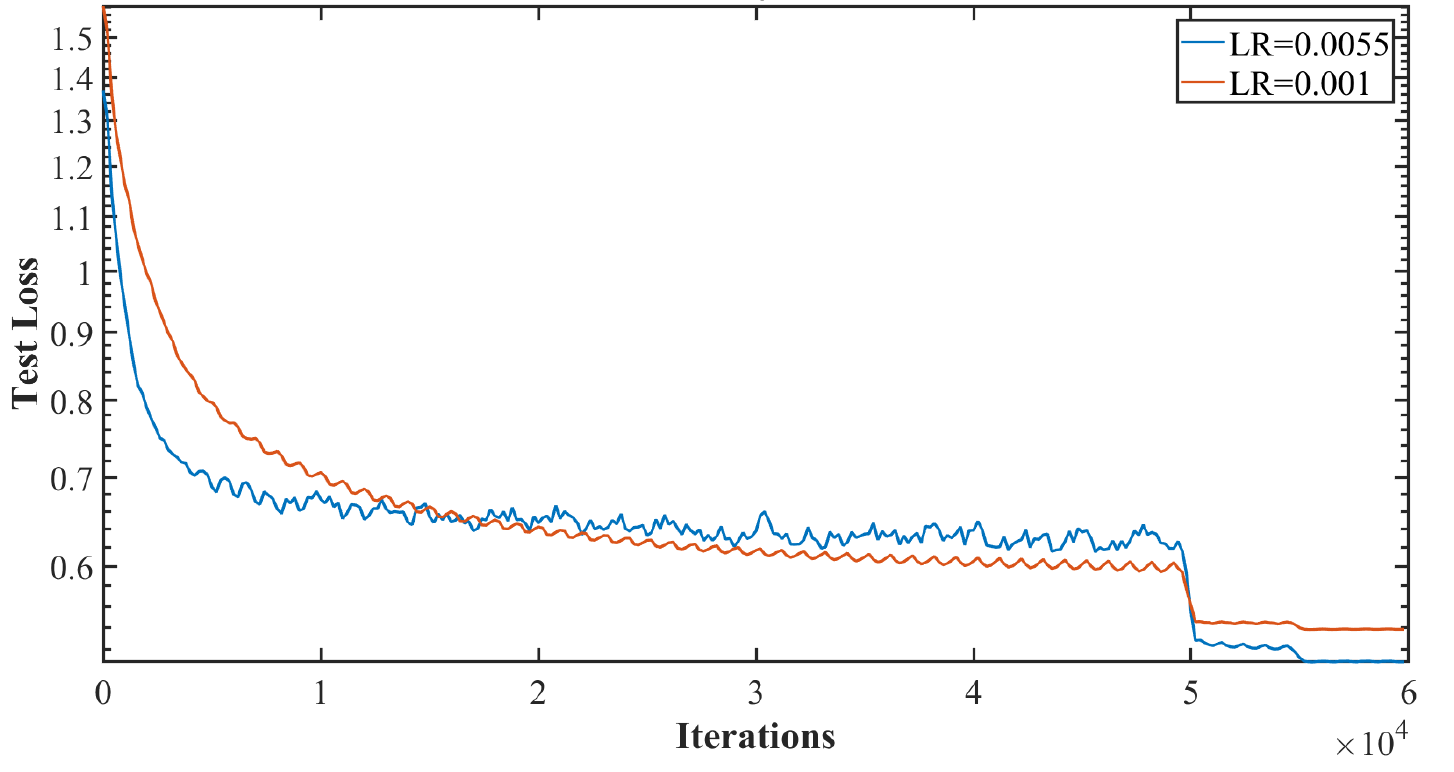
\includegraphics[width=0.50\textwidth]{Bilder/underfitting.png}
\captionsetup{width=0.50\textwidth}
\caption{Underfitting: Validation / Test Loss of a model training with a learning rate of 0.005 and 0.001 taken from \cite{DBLP:journals/corr/abs-1803-09820}.}
\label{underfitting}
\end{wrapfigure}

\textbf{Underfitting} is the inability of a model to decrease the error of the training or a validation set. It is implying that the model is not able to solve the underlying complexities of the data distributions. It further is characterized by a steadily decreasing validation loss instead of a more horizontal line. The practitioner can increase the learning rate to reduce Underfitting. The concept of underfitting can be seen at \figref{underfitting}, which is the result of a 3 layer network training on the Cifar10 \cite{cifar} dataset taken from \cite{DBLP:journals/corr/abs-1803-09820}.\\

\textbf{Overfitting} occurs if a model is doing excessively well on the training set with an increasing generalization error. The generalization error can be calculated by subtracting the training loss from the validation loss. While a steadily decreasing validation loss can often recognize Underfitting, Overfitting seems to be more complicated. In the left image of \figref{overfitting}, a result from a learning rate test can be seen, where models, depending on three different weight decays, start to overfit at a learning rate of 0.002 for the blue, 0.005 for the yellow, and 0.008 for the red line. At the right image, which has a steady learning rate set, the smaller weight decay also causes the orange model's validation loss to increase. In contrast, the blue model rather underfits, with a decreasing validation loss.

 \begin{figure}[h]%[htbp]
\centering
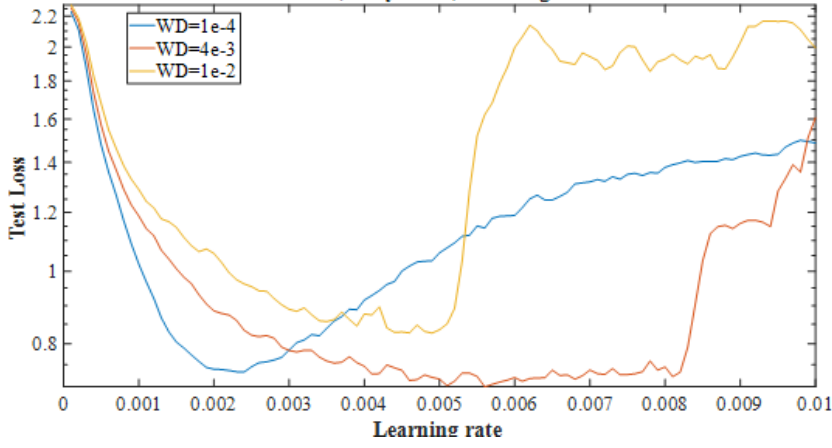
\includegraphics[width=0.45\textwidth]{Bilder/learning_rate_test.png} 
\hspace{1.0 cm}
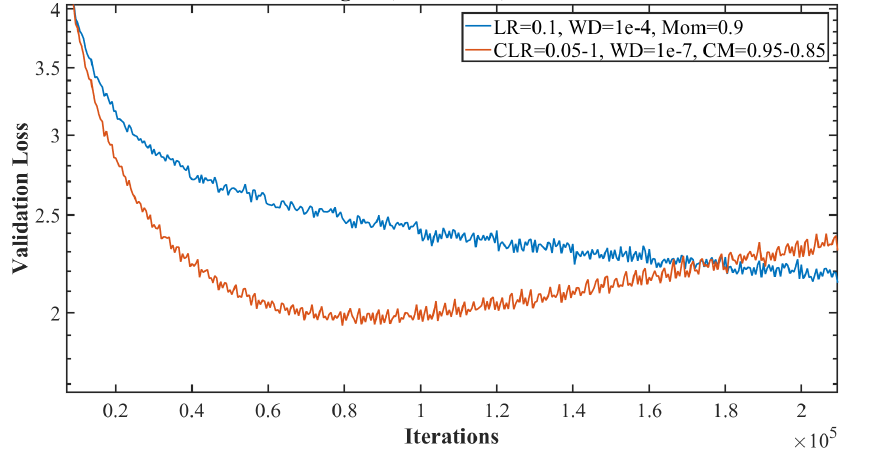
\includegraphics[width=0.45\textwidth]{Bilder/overfitting_underfitting.png} 
\caption[]{The left image shows a learning rate test result with models swapping from under, to overfitting for a specific learning rate. The right image depicts two models with different weight decays, where the one with the smaller value, tends to overfit. The images are taken from the paper \cite{DBLP:journals/corr/abs-1803-09820} and display results from the training on Cifar10 \cite{cifar} and Imagenet \cite{imagenet_cvpr09}.}
\label{overfitting}
\end{figure}

\begin{wrapfigure}{R}{0.45\textwidth}
\centering
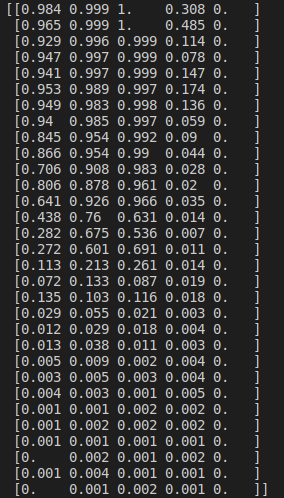
\includegraphics[width=0.35\textwidth]{Bilder/numpy_pred_shape.png}
\captionsetup{width=0.35\textwidth}
\caption{Model output displaying the predictions for distances (rows) and laser ranges (columns), given raw image data as input. The prediction shows that an obstacle is detected in the left upper corner. The probabilities in this area, are all around $1$.}
\label{numpy_pred_shape}
\vspace{5pt}
\end{wrapfigure}

To directly compare the validation versus the training loss, a graph, as depicted in the left image of \figref{train_val}, is extracted directly from the training process. Due to \cite{Goodfellow-et-al-2016}, the training and validation loss can further give some insight into whether underlying software is implemented correctly. The author claims that if the training error is low, but the test error is high, it is likely that the training procedure is implemented correctly. The model overfits, due to different reasons like a software error.

\textbf{The Learning rate} is considered the most important parameter by \cite{Goodfellow-et-al-2016}. He suggests tuning the learning rate if time is scarce exclusively. This is due to the effective capacity which this hyperparameter controls. He claims that if the learning rate is properly set, the effective capacity is highest, whether the learning rate is excessively low or large.

\begin{figure}[H]%[htbp]
\centering
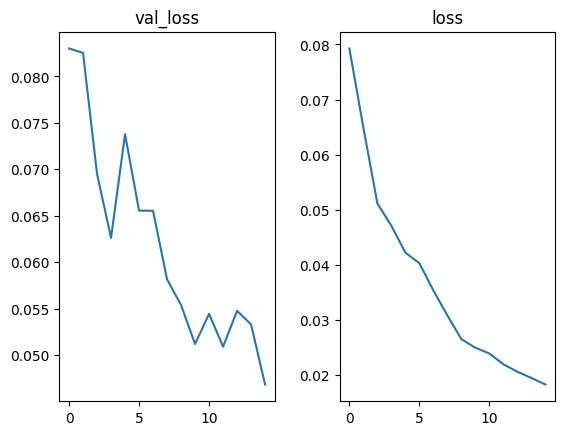
\includegraphics[width=8cm,height=6cm]{3_models/models_10/graph_10.png}
\hspace{0.2 cm}
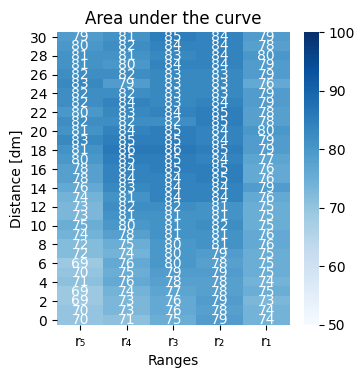
\includegraphics[width=6cm,height=6cm]{4_plots/plots_10/AUC_10.png}
\caption{The left graph shows the validation versus the training loss while the right graph shows the summary of the Area Under the Receiver Operating Characteristic curve for all ranges from $\{r_{1}, ... ,r_{n}\}$ as well for all intermediary positions (distances).}
\label{train_val}
\end{figure}

\subsubsection{Simulation prototype \label{sim_prototype} }
The trained model is further used as a prototype in simulation. The following tests will be documented for each model. 

\begin{itemize}
\item Recognition of unknown obstacles
\item Recognition of empty areas
\item Recognition of correct distances
\item Recognition of correct laser ranges
\end{itemize}

It is important to note that for this part, no validation data can be used. As input, the model is given raw data from the camera. The prediction is an array, transformed to a shape of the form depicted in \figref{numpy_pred_shape}, where each column stands for a laser range and each row for an intermediary position (distances). The first row at the top predicts obstacles that are the furthest away from the camera, while the last row predicts the closest obstacles.\\


\textbf{Unknown obstacles}\\
It is documented whether the model can efficiently predict obstacles it has not been trained with. The unknown obstacles can have different shapes, be positioned differently, or display different colors.\\

\textbf{Empty areas}\\
Here it is tested whether the model can recognize areas without obstacles. Decreasing the failure rate at this step, the parameter, which decides how many empty instances are recorded, can be adjusted as discussed in \secref{DataAcquisition}.\\

\textbf{Correct distance}\\
At this step, it is tested whether the distance predicted seems to be accurate. Objects at the furthest position and objects that stand right in front of the camera are being tested. In \figref{numpy_pred_shape}, the distances stand for each row. The first row at the top predicts obstacles that are the furthest away from the camera.\\

\textbf{Correct laser range}\\
Here the columns of \figref{numpy_pred_shape} are tested for consistency. This step also can be tested in combination with the correct distance. This step and the previous are also important to figure out the most efficient thresholds discussed at \secref{FeatureExtraction}, to define the number of laser ranges or the distance in which obstacles around the robot are considered as relevant for the creation of the dataset.\\

\subsubsection{Visualizing model \label{visualizing} }
This part is about the creation of a short video, given a bagfile and dataset as input. Like the heatmap output, the video can provide a representable visualization file of the prediction concept. Videos at this step can be created for every bagfile in combination with a model. Except for the trajectory covered by the robot, the video additionally contains the predictions made by the model for the given recording. The concept of this algorithm is provided by \cite{nava2019learning}.\\

It is generally recommended to visualize the model in action. \cite{Goodfellow-et-al-2016} suggests that it helps to determine whether the quantitative performance numbers are reasonable. Especially bugs that give no error message might be reduced by visualization, due to the author. He further claims that not only can visualization help to discover the presence of a bug. It also can give hints about its localization.

\subsubsection{File Administration \label{file_administration} }
This section is about the administration of files created and used throughout this project. As depicted in \figref{pipeline}, every stage is given a file as input, while creating another file as output. To provide coherence, flexibility, and consistency over the entire pipeline process, a File Administration Class is proposed, which covers the following tasks:

\begin{itemize}
\item Consistent and unique folder and file structure for each pipeline run
\item Mechanisms to reuse files
\item Data verification
\item Autonomous parameter and test result documentation
\end{itemize}

\textbf{Folder and File structure}\\
To provide usability, flexibility, and a fully autonomous process, the proposed class implements an efficient file and folder structure, which stores and names the files to relate or distinguish them from each other, throughout the entire pipeline run. An additional custom error class indicates if files are erroneous, missing, or attempted to be overwritten.\\

\textbf{Reuse files}\\
Specific pipeline stages can be skipped to save time and resources. If several recorded bagfiles exist already, they can be reused from previous runs and adequately incorporated into the current pipeline. File or folder names are automatically changed to fit the new pipeline run.\\

\textbf{Data verification}\\
Data verification is an essential part of every machine learning pipeline to prevent erroneous data from being passed to the next stage. Files may contain incomplete data or provide duplicates, which might cause subsequent stages to fail. As it is hard to predict all eventualities, it is also hard to implement all data verification mechanisms in advance. The following mechanisms are currently implemented to verify files and data:

\begin{itemize}
\item Prevention to pass unfinished recordings to Feature Extraction
\item Mechanism to erase duplicates in bagfiles
\item Wrong data types set over the entire pipeline
\item Prevention of an erroneous folder or file structure
\end{itemize}

\textbf{Documentation}\\
To increase usability and avoid redundant tasks, the pipeline stores and documents the tests and parameters used at every pipeline stage. The output format is set to Markdown and Latex. Most of the experimental results of the file \path{ss20_lanz_2d_obstacle_avoidance/doc/thesis/Thesis_appendix.pdf}, are autonomously created by the pipeline.

\newpage
\subsection{Obstacle Avoidance Controller \label{o_a_controller} }
This final part of the implementation proposes an obstacle avoidance controller. The goal is to provide the trained model with raw images from the robot's camera and use its prediction to avoid obstacles on a path towards a goal reliably. To test the deployment, the same framework, as described in \secref{framework}, is used. As a first test scenario, the implementation proposes to set up some predefined coordinates, where the robot can maneuver in a loop. Obstacles can then be put along the path to test whether the controller can avoid them efficiently. \figref{deployment_scenario} displays such a scenario, with objects along the path, the robot has to avoid.

Following list further specifies necessary steps to obtain a fully autonomous obstacle avoidance controller for this project, with each of them being discussed in more detail in the subsequent subchapters:

\begin{itemize}
\item Conversion of \textbf{model output} to a convenient form
\item Development of basic \textbf{trajectory functionalities}
\item Implementation of an \textbf{obstacle avoidance algorithm}
\item Real time heatmap for \textbf{visualization}
\end{itemize}

\begin{figure}[h]%[htbp]
\centering
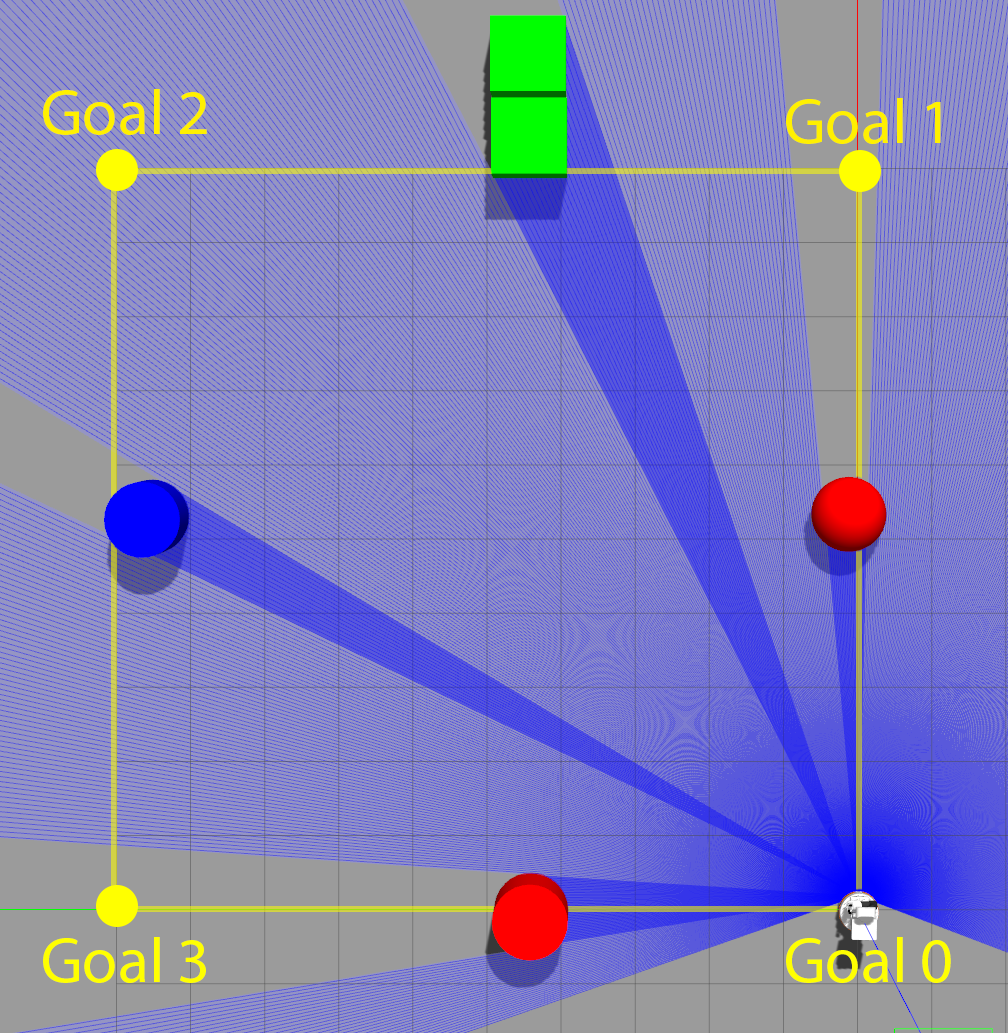
\includegraphics[width=0.48\textwidth]{Bilder/deployment_scenario.png} 
\caption[]{Simple scenario with four goals and obstacles along its trajectory.}
\label{deployment_scenario}
\end{figure}

\subsubsection{Model Output \label{model_output} }
The output of the model, given an image, always has the form of a one-dimensional array. The length of the output array depends on the number of laser-ranges and the number of intermediary positions used. Taking the example dataset from table \ref{tab:example_prediction}, the model output would have 15 elements or more generally

\begin{equation}
\label{eqn:10}
o_{len} = p_{len} * r_{len}
\end{equation}

where $p_{len}$ stands for the number of intermediary positions and $r_{len}$ for the amount of laser ranges used.\\

To provide a more convenient way for the development of an obstacle avoidance controller, it makes sense to reshape the array from $shape(o_{len},)$ to $shape(p_{len},r_{len})$. An example of such a reshaped array can be seen in \figref{numpy_pred_shape}. The example array has the shape of $(31,5)$, where columns stand for laser-ranges, and rows for distances. Therefore, each array's element predicts a distance and information about the corresponding angular position of a possible obstacle in front of the robot. If the prediction is zero or close to zero, the model predicts no obstacle at the element's position. Interpreting \figref{numpy_pred_shape}, several elements at the left upper corner predict an obstacle with a distance of about 3 meters from the robot's position. The corresponding image would also display one or several obstacles at the left upper corner.\\

A shape in such a form can then serve as the input of an obstacle avoidance controller, further described in the next subchapters.

\subsubsection{Trajectory functionalities \label{trajectory_functionalities} }
To have a robot maneuver a simulation environment, it is essential to have a set of basic trajectory functionalities. Following basic functions have been defined or ajusted for this part of the implementation:

\begin{itemize}
\item MoveTowardsGoal()
\begin{itemize}
\item CalculateAlternativeAtan2()
\item CalculateAlternativeTheta()
\item CalculateAngularVelocity()
\end{itemize}
\item CalculateEuclideanDistance()
\item Greenlight()
\item TransferCoordinate()
\end{itemize}


\begin{wrapfigure}{R}{0.45\textwidth}
\centering
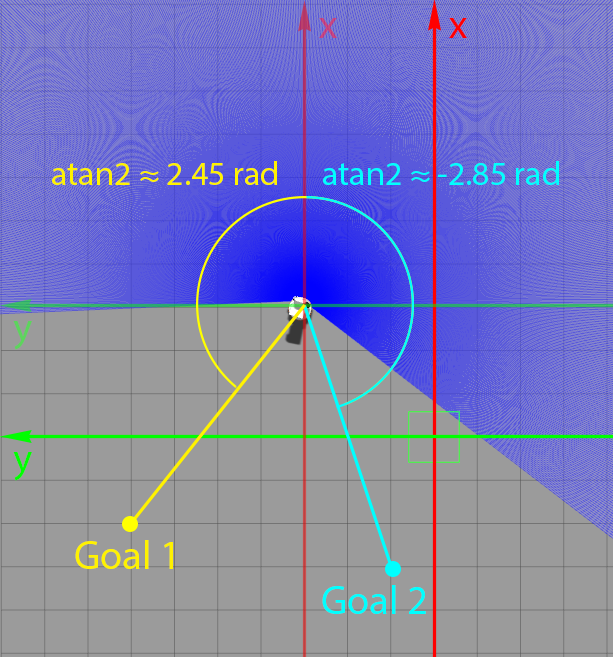
\includegraphics[width=0.35\textwidth]{Bilder/atan2.png}
\captionsetup{width=0.35\textwidth}
\caption{Concept of $\atantwo(y,x)$ with a standard range from $0$ to $\pi$ for the first and second quadrant and from $-\pi$ to $0$ for the third and fourth quadrant.}
\label{atan2}
\vspace{10pt}
\end{wrapfigure}

\textbf{Move towards goal}\\
This function's concept is similar to turning for a specific degree around the robot's axis, described in detail in \secref{statemachine} at state 5 of the state machine. Instead of directly calculating with a fixed angle to turn, an additional value obtained from the function $\atantwo(y,x)$ needs to be observed at this step. $\atantwo(y,x)$ provides the angle from the robots x-axis, parallel to the x-axis of world coordinates, and the goal position. The concept of $\atantwo(y,x)$ can be seen in \figref{atan2}. The function takes as parameters coordinates from the robot's own and the desired goal position. The function is defined from $0$ to $\pi$, for the first and second quadrant, and from $-\pi$ to $0$, for the third and fourth quadrant. This definition can cause a similar problem with the robot getting caught in a flipping state, described in \secref{statemachine}. To provide a more robust and smooth implementation, $\atantwo(y,x)$ and $\theta$ are both mapped to a range from $0$ to $2\pi$. The advantage of such a mapping is that just one flip, instead of 2, must be observed. A flip in this context means a non-fluent change of input values, like from $\pi$ to $-\pi$. An example of this concept for $\theta$ can be seen in \figref{theta_alt} where $\theta$ is mapped to a range from $0$ to $2\pi$. The following case statement calculates the angular velocity, where the corresponding function can feed the output directly to the robots  motion sensors:

\begin{equation}
\label{eqn:11}
\resizebox{.90\textwidth}{!}{$\displaystyle
V(\theta_{alt},atan2_{alt}) =
\begin{cases}
atan2_{alt} + 2\pi - \theta_{alt}, &\{\theta_{alt},atan2_{alt}|atan2_{alt} - \theta_{alt} < -\pi \}\\
atan2_{alt} - 2\pi - \theta_{alt}, &\{\theta_{alt},atan2_{alt}|atan2_{alt} - \theta_{alt} > \pi\}\\
atan2_{alt} - \theta_{alt}, &{otherwise }
\end{cases}
$}
\end{equation}

\figref{move_to_goal} displays the first case of equation \ref{eqn:11} at the left and the second case of equation \ref{eqn:11} at the right. The third case is applied otherwise.\\

The result $ V $ can then be fed directly to the robot's motion sensor to turn the robot to some desired goal coordinates. 

\begin{figure}[h]%[htbp]
\centering
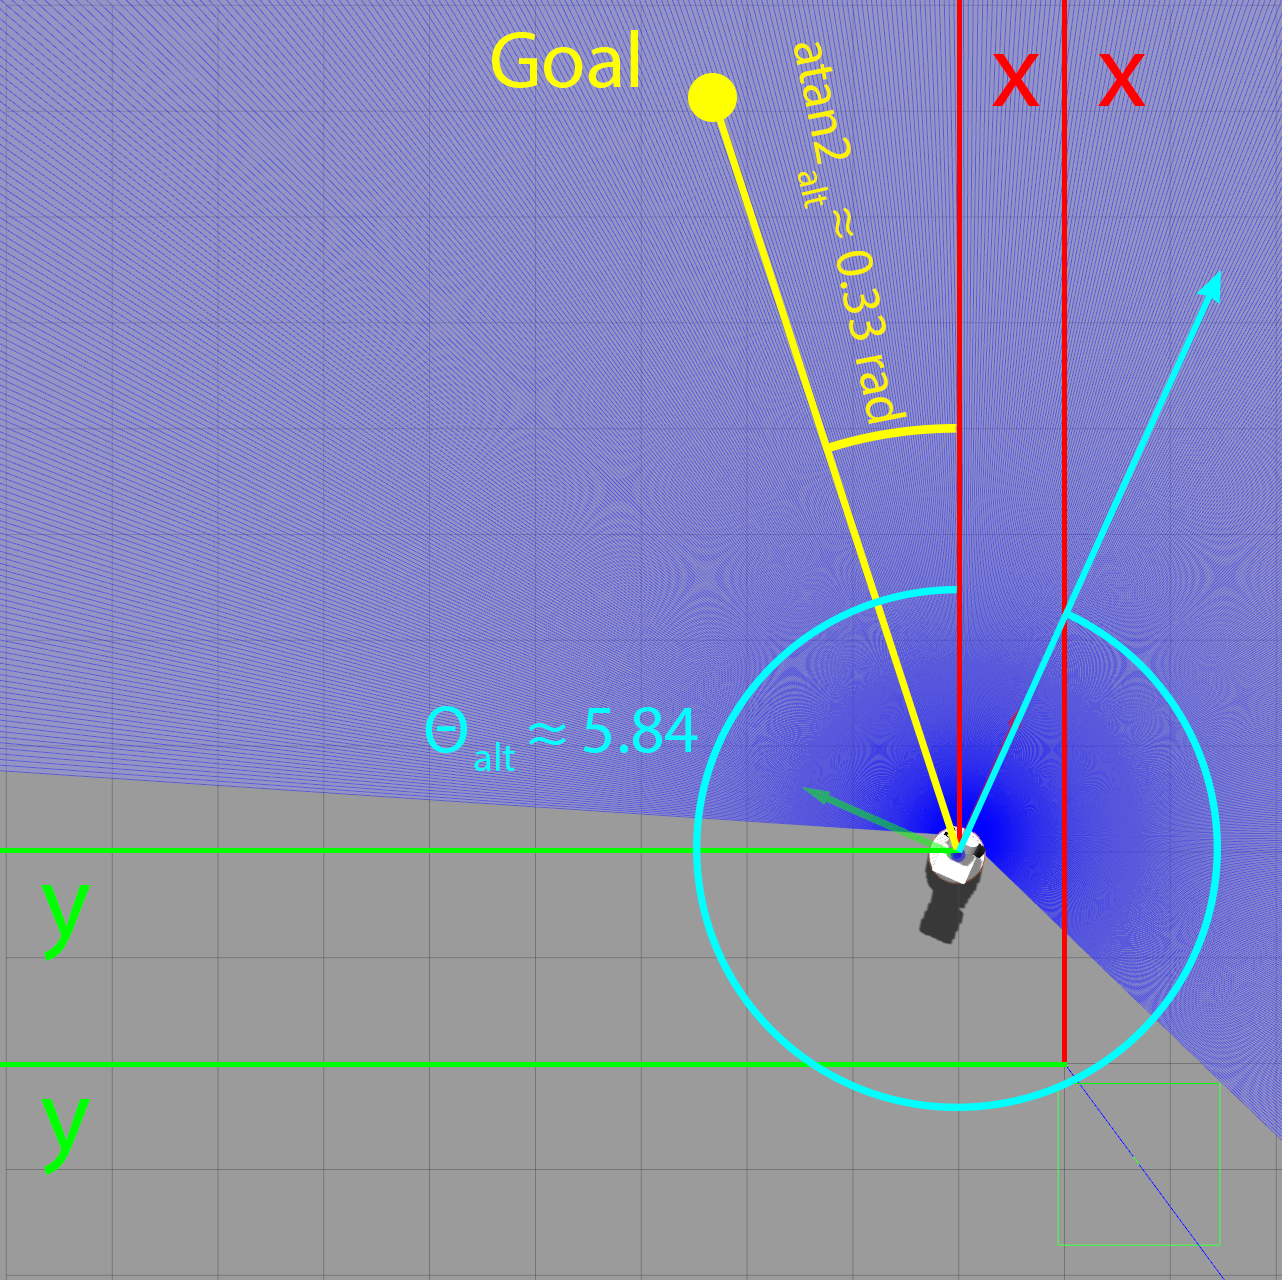
\includegraphics[width=0.48\textwidth]{Bilder/move_to_goal_case_1.png} 
\hspace{0.2 cm}
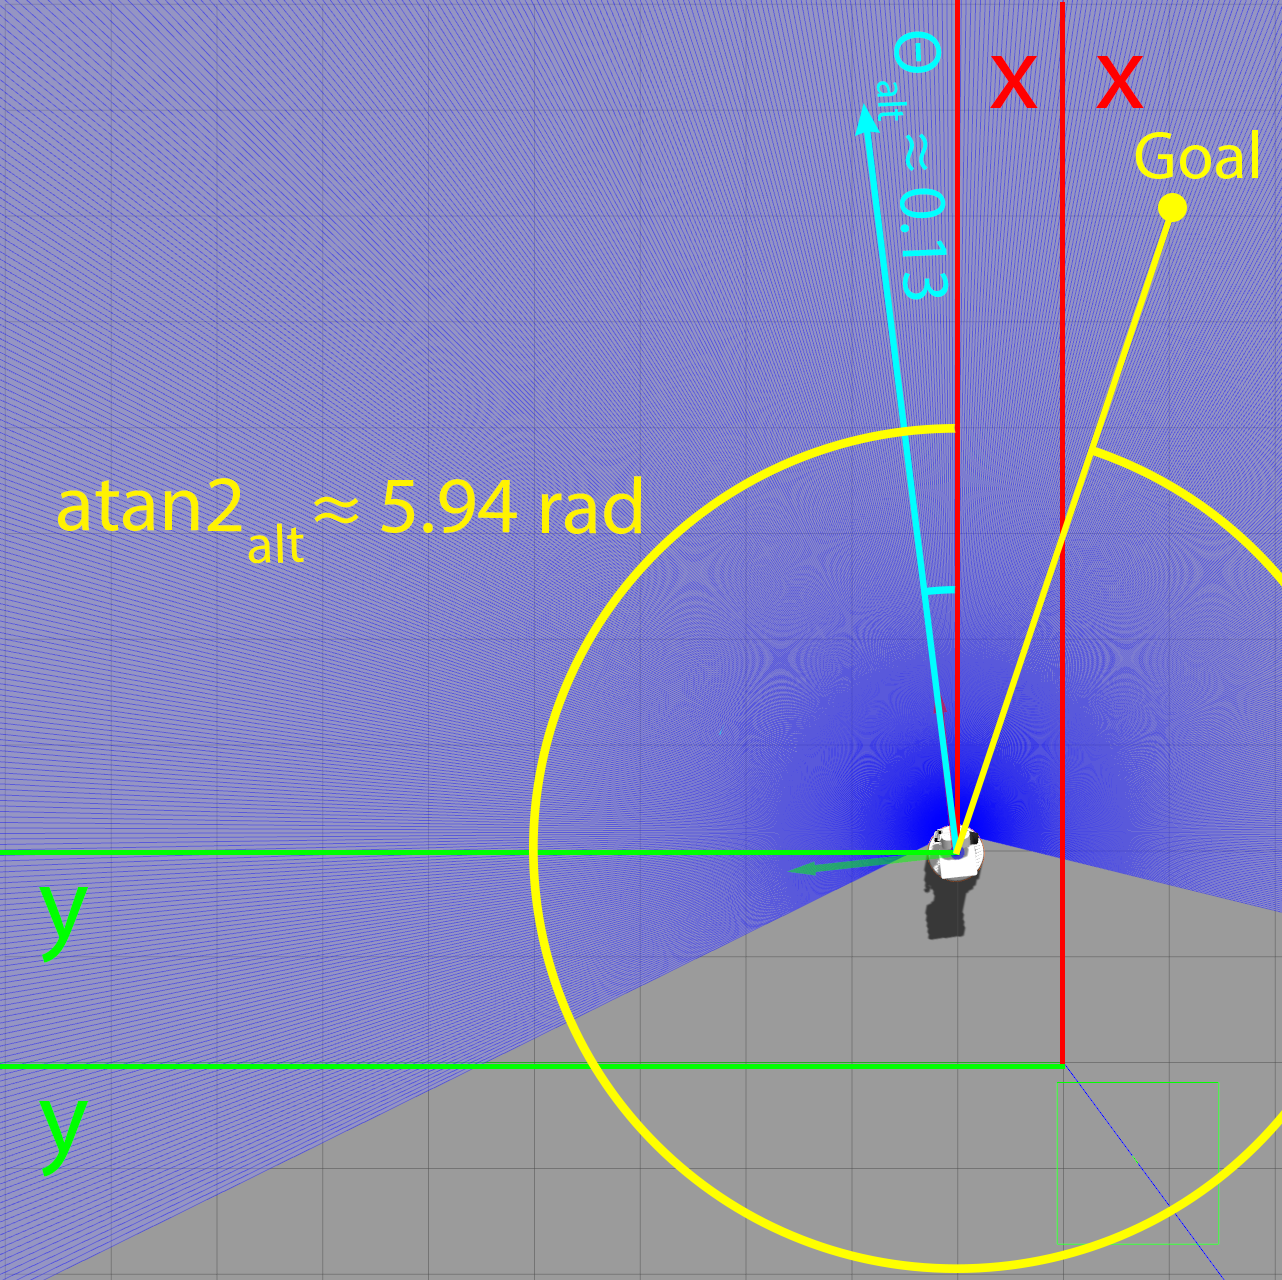
\includegraphics[width=0.48\textwidth]{Bilder/move_to_goal_case_2.png} 
\caption[]{The left image displays a situation where the first case of equation \ref{eqn:11} is applied as $atan2_{alt} - \theta_{alt}$ is way smaller than $-\pi$, while the right image shows a situation where the second case is applied as $atan2_{alt} - \theta_{alt}$ is much bigger than $\pi$. Both cases, then would lead the robot turning to the right direction towards the goal.}
\label{move_to_goal}
\end{figure}

\textbf{Euclidean Distance}\\
To calculate the distance between the robots own position $p_{robot}$ and a goal position $p_{goal}$, following formula can be implemented
\begin{equation}
\label{eqn:12}
{\displaystyle {\begin{aligned}d(\mathbf {g} ,\mathbf {p} )&={\sqrt {(g_{1}-p_{1})^{2}+(g_{2}-p_{2})^{2}}}\\[8pt]&={\sqrt {\sum _{i=1}^{2}(g_{i}-p_{i})^{2}}}.\end{aligned}}}
\end{equation}

This function can be used in various situations. One use case is to check whether the robot reaches a specific goal. As it is often not necessary to be precisely on a goal position, a threshold around a specific goal area can be defined, where a function returns True, once the robot reached the defined threshold. The advantage of this is to prevent the robot from overshooting the desired goal by odometry drift.\\

\textbf{Greenlight}\\
This functionality translates the model's output, described in \secref{model_output}, to a desired number of areas, to achieve a more convenient format for an obstacle avoidance algorithm to use.\\  

One proposal used for this project is to divide the transformed model output, as in \figref{numpy_pred_shape} or \figref{heatmap}, in up to three zones, where the first and second column are defined as the left, the center column as the mid, and the fourth and fifth column as the right zone. With the mean taken from each zone, a simple but efficient prediction can be achieved to decide whether an obstacle hits a zone or not. A threshold can be defined to decide whether the mean is considered as True (Obstacle detected) or False (No obstacle detected). As there are two possibilities for three zones, the total number of outputs to observe is

\begin{equation}
\label{eqn:13}
N = 2^3 = 8
\end{equation}

\secref{obstacle_avoidance} describes in more detail how an obstacle avoidance controller can react to the greenlight outputs given.\\

\textbf{Transfer coordinate}\\
As described in \secref{state_machine} with the equation \ref{eqn:4}, this part uses the concept of transferring coordinates from one system to another. Following equation transfers a robot coordinate $\vec{P}_{g}$ to a world coordinate $\vec{P}_{g_{world}}$

\begin{equation}
\label{eqn:13} 
\vec{P}_{g_{world}}=
\vec{P}_{g}*
  \begin{bmatrix}
    \cos(\alpha) & -\sin(\alpha)\\
    \sin(\alpha) & \cos(\alpha)
  \end{bmatrix}+
\vec{P}_{r_{world}}
\end{equation}

\secref{obstacle_avoidance} further describes how this function can be made of use by an obstacle avoidance controller.

\subsubsection{Obstacle avoidance algorithm \label{obstacle_avoidance}}
This subsection describes the Bug algorithms and a modified version of an intermediary goal algorithm. Both algorithms have their advantages and disadvantages, and both are tested using the trained model's output as the necessary visibility sensor.\\

\textbf{Bug Algorithms}\\
The Bug, Bug2, and VisBug algorithms are described in much more detail by \cite{lavalle2006planning} in the chapter "Planning in Unknown Continuous Environments." The author describes the necessary robot configuration to implement such an algorithm as follows:

\begin{quote}{Steven M. LaValle}
\begin{itemize}
\item  A goal sensor indicates the current Euclidean distance to the goal and the direction to the goal, expressed concerning an absolute "north."
\item A local visibility sensor provides the exact shape of the boundary within a small distance from the robot. The robot must contact or almost contact to observe part of the boundary; otherwise, the sensor provides no useful information.
\end{itemize}
\end{quote}

As the simulation provides coordinates about the robot's position, the Euclidean distance can be calculated as in equation \ref{eqn:12}. This concept leads to the first of Steven M. LaValle's requirements to be met. As for the second requirement, the model's output can be used as a visibility sensor, as it provides all the necessary information needed about the robot's environment. \figref{Bug} describes both strategies where the strategy at the right (Bug2) has a much better performance.

\begin{figure}[h]%[htbp]
\centering
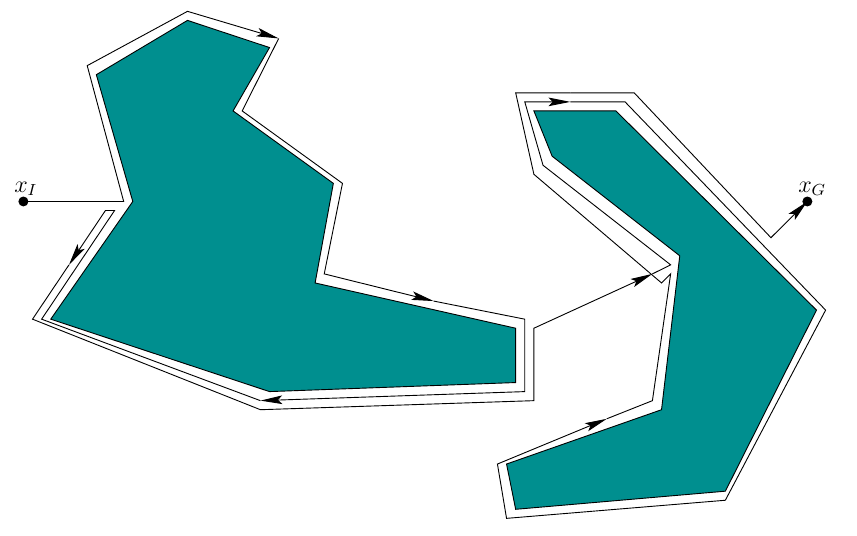
\includegraphics[width=0.48\textwidth]{Bilder/Bug1.png} 
\hspace{0.2 cm}
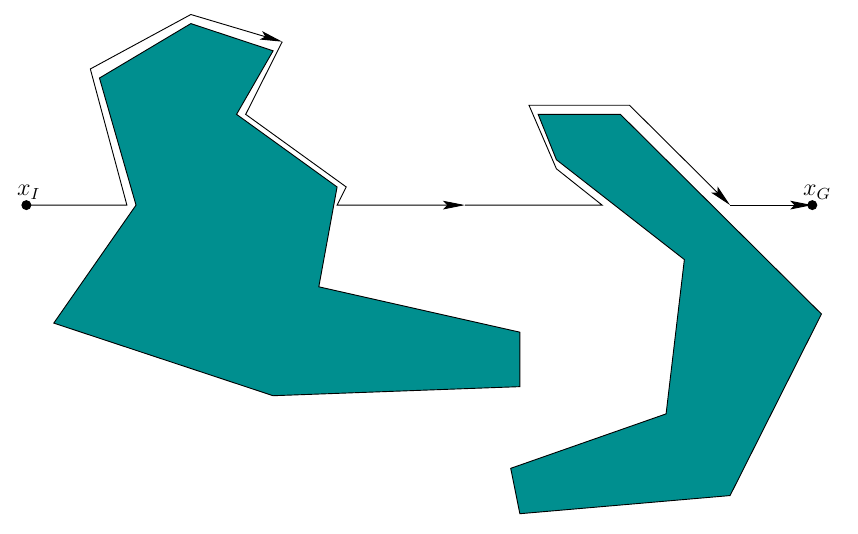
\includegraphics[width=0.48\textwidth]{Bilder/Bug2.png} 
\caption[]{Graph displaying the Bug concept from \cite{lavalle2006planning}. Bug1 (left image) and Bug2 (right image) strategy, with major performance gain in favor of Bug 2. }
\label{Bug}
\end{figure}

As both Bug1 and Bug2's performance is not entirely satisfying, a third algorithm called VisBug seems to be rather promising to test. \figref{visbug} shows the concept of VisBug. The difference is that instead of finding a straight line to the goal, VisBug continually checks if the direction towards the goal is free of obstacles. If that is the case, the robot immediately heading towards the goal. This functionality further increases performance over Bug2, in favor of VisBug.\\

\begin{figure}[h]%[htbp]
\centering
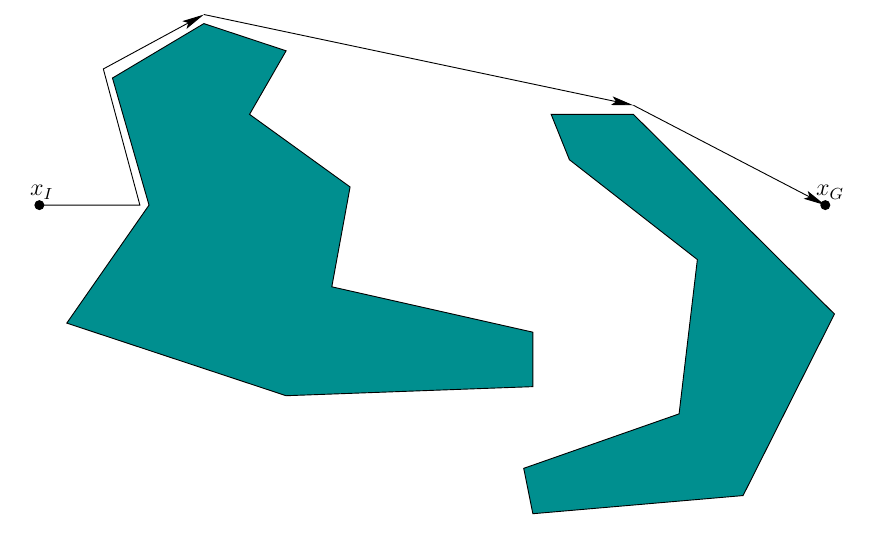
\includegraphics[width=0.48\textwidth]{Bilder/visbug.png} 
\caption[]{Concept of VisBug taken from \cite{lavalle2006planning}}
\label{visbug}
\end{figure}

The disadvantage of Bug1 and Bug2 is its performance and for VisBug, the fact that it continually needs to check whether the path towards the goal is free of obstacles. The robot is continuously turning towards a goal, while in the next instance, turning away to avoid it. This behavior requires the model's output, especially the outer ranges, to provide an extremely accurate performance. At this step, it is essential to note that the camera's view is limited to a fixed angle, which makes it nearly impossible to implement such an algorithm properly. The camera's field of view, and the resulting visibility sensor, are not wide enough. An additional, more robust algorithm is tested and described next.\\

\textbf{Intermediary Goal Algorithm}\\
The concept of a possible intermediary goal algorithm is described in \cite{doi:10.1177/1729881418759107}. This algorithm is laser-based, but the concept can partially be applied for a visibility sensor provided as the model's output. The paper proposes several steps to find the perfect intermediary goal if the sensor senses an obstacle around the robot's vicinity. The steps to find the perfect intermediary goal are described below. It is important to note that before the steps are applied, the entire range of lasers in front of the robot are considered as possible intermediary goal candidates. By following the steps, the number of candidates decreases until the best one is found. \figref{laser_based} displays this concept.

\begin{figure}[h]%[htbp]
\centering
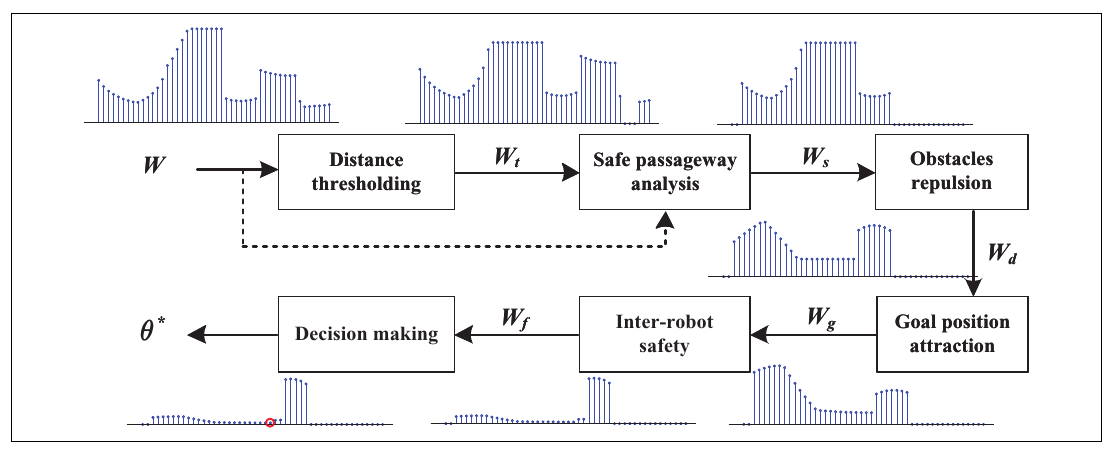
\includegraphics[width=1\textwidth]{Bilder/laser_based.png} 
\caption[]{Concept of an Intermediary Goal Algorithm taken from \cite{doi:10.1177/1729881418759107}}
\label{laser_based}
\end{figure}

\begin{itemize}
\item  \textbf{Distance thresholding} erases all intermediary goal candidates, which point to the same direction as obstacles under a certain threshold. This means that if an obstacle is detected less than a specific distance from the robot, all goal candidates with the same direction are considered invalid.
\item  \textbf{Safe passageway analysis} further analyzes all remaining goal candidates, calculating a safe passage for all directions similar as described in \secref{state_machine}. The remaining possible candidates are then given to the next step.
\item  \textbf{Obstacle repulsion} artificially increases the distance of remaining risky goal candidates to give them less weight for the next step.
\item  \textbf{Goal position attraction} applies a function on the remaining candidates to chose a direction convenient to the direction of the primary goal. All other candidates are erased, and the remaining ones passed to the next step.
\item  \textbf{Inter-robot safety} analyzes other robots  close by and erasing goal candidates with the highest risk.
\item  \textbf{Decision making} applies a function on the remaining intermediary goal candidates, returning a weight for each direction. The direction with the lowest weight can then be chosen as the final intermediary goal.
\end{itemize}

While this concept is developed for a laser-based approach, it can be partially applied to the current project. \textbf{Distance thresholding} can be directly applied to the output and the concept of \textbf{Safe passageway analysis} is calculated by the mean of a range and distance combination. \textbf{Obstacle repulsion}, \textbf{Goal position attraction}, \textbf{Inter-robot safety} and \textbf{Decision making} are combined and used slightly different.\\

As mentioned in \secref{trajectory_functionalities} under the paragraph "Greenlight", the outputs of the function implemented are a set of 8 possible combinations. This concept is used for one of the following versions to calculate a possible intermediary goal candidate if obstacles interfere with the robot's camera field of view. As follows, two versions for an intermediary goal obstacle avoidance controller are presented.\\


\textbf{1. Version}\\
Following version uses the greenlight concept described in \secref{trajectory_functionalities}. The greenlight function simplifies the model's output to three ranges with eight combinations. The following list describes the functions outputs and their corresponding reactions.
\begin{itemize}
\item  \textbf{False, False, False} Here, the prediction's output does not recognize any obstacles close by. The robot can keep moving towards a desired goal.
\item  \textbf{False, False, True} This output indicates an obstacle recognized at the cameras field's right edge. To avoid collisions, an intermediary goal, which is located at the outer left, can be chosen. 
\item  \textbf{False, True, True} Similar to the previous output, the intermediary goal at this step is located towards the left of the robot's own position. The robot's angle towards the goal needs to be greater than in the previous step.
\item  \textbf{True, False, False} This output's reaction is similar to the reaction to the second, with an intermediary goal located towards the right instead of the left.
\item  \textbf{True, True, False} The reaction to this output is also equal to the previous with the intermediary goal located towards the right but with a greater angle.
\item  \textbf{True, False, True} At this output, obstacles at the right and left, but no obstacles in front of the robot are detected. To avoid collision and decide whether the middle area is wide enough for the robot to pass, all output ranges need to be observed. The "Greenlight" function, described in \secref{trajectory_functionalities} combined the outer columns to reduce the number of outputs from $N = 2^5 = 32$ to $N = 2^3 = 8$. For this output, a more precise distinction is required to find a possible intermediary candidate to decide whether to pass through the middle or not. This result can be achieved by calculating the prediction's mean for the second and fourth column. If their mean is close to zero, no intermediary goal needs to be calculated. If their mean is above a certain threshold, it is necessary to choose an intermediary goal with an angle greater than 45 degrees.
\item  \textbf{False, True, False} At this output, the intermediary goal can be located at the left or right. The means of the left and right zone can be compared to find the safest intermediary goal for the robot navigate to.
\item  \textbf{True, True, True} If obstacles are all around the robot's camera field of view, the intermediary goal's degree needs to be greater than 45 degrees. Even an angle of 90 degrees can be considered, as the obstacle in front could be a wall. Once the intermediary goal is reached, the prediction could be re-evaluated.
\end{itemize}

Once the intermediary goal is reached, the robot turns back towards the primary goal, analyzing the environment for obstacles in front of it, again.\\

This version's disadvantage is the "Greenlight" functionality, which uses three, instead of all $n$ ranges available. It would be possible to use all $n$ ranges, increasing the combinations to $N = 2^n$. In the case of 5 ranges used, the combinations would be 32. As the "Greenlight" functionality reduces the output, it lacks accuracy by combining two ranges. The concept of this mechanism, is described in \secref{trajectory_functionalities}. A second version, which is easier to maintain, is implemented and described as follows.\\

\textbf{2. Version}\\
As the first version revealed some disadvantages in accuracy and flexibility, a subsequent version is implemented at this step.\\

A greenlight, or safe passage for the robot is considered if the lower part of the prediction does not exceed a specific threshold. The number of rows to take into consideration is flexible. As more rows are chosen, as earlier, the threshold is exceeded with the controller displaying a higher sensitivity. The concept of this can be seen at \figref{intermediary_goal}, where the threshold is set to the first 15 rows. If these row's mean does not exceed a minimal value, the robot is free to move forward. If the mean below that threshold is exceeded, the robot needs to immediately slow down while analyzing all ranges as their whole by calculating their corresponding mean.\\

Depending on the result, which is given as an array of $n$ values, where n stands for the number of ranges used, a decision about the best intermediary goal position can be suggested. \figref{intermediary_goal} further describes this concept, where an intermediary goal is chosen based on each prediction range's weight.\\ 

In the left image, all ranges show a very high probability of obstacles. Therefore, the intermediary goal has to be chosen below the defined threshold, as the object could be a wall. Once the intermediary goal is reached, the prediction needs to be re-evaluated.\\

In the right image, the intermediary goal can be chosen above the threshold. This type of avoidance is just possible if both of the outer ranges are predicted as obstacle-free zones. If just one of the outer ranges is predicted as free, the intermediary goal should also be set below the threshold, similar to the first image.



\begin{figure}[h]%[htbp]
\centering
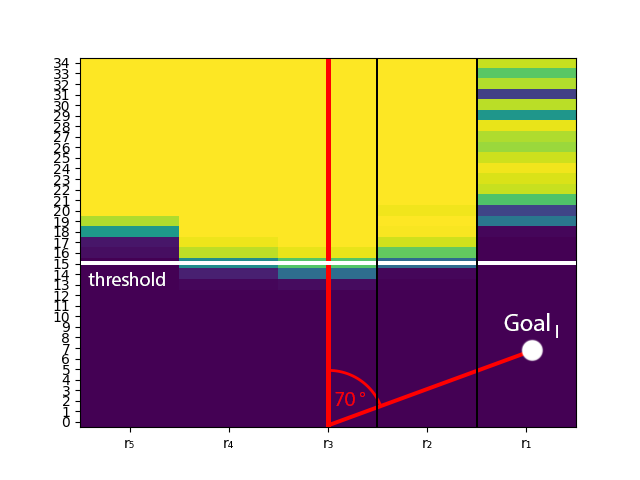
\includegraphics[width=0.48\textwidth]{Bilder/intermediary_goal_1.png} 
\hspace{0.2 cm}
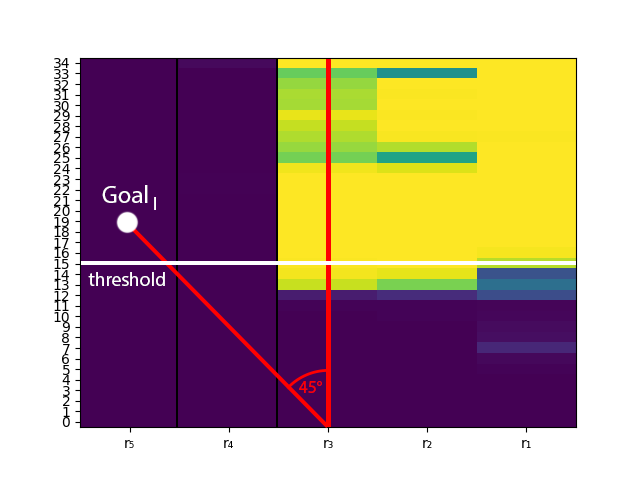
\includegraphics[width=0.48\textwidth]{Bilder/intermediary_goal_2.png} 
\caption[]{Images indicating the direction of a possible, intermediary goal candidate. At the left image, the intermediary goal has to be located below the threshold as the obstacle could be a wall, while at the right image, the intermediary goal can be located above the threshold. Once the intermediary goal is reached. The prediction needs to be re-evaluated.}
\label{intermediary_goal}
\end{figure}
\newpage

\subsubsection{Visualization \label{visualization} }
To provide a visual representation in real-time about the model's prediction, a heatmap depicted in \figref{heatmap} is created. The map is a great tool to analyze the performance intuitively and fix or adjust parameters to increase performance. Visualization is generally recommended and also discussed further in \secref{visualizing}.

\begin{figure}[h]%[htbp]
\centering
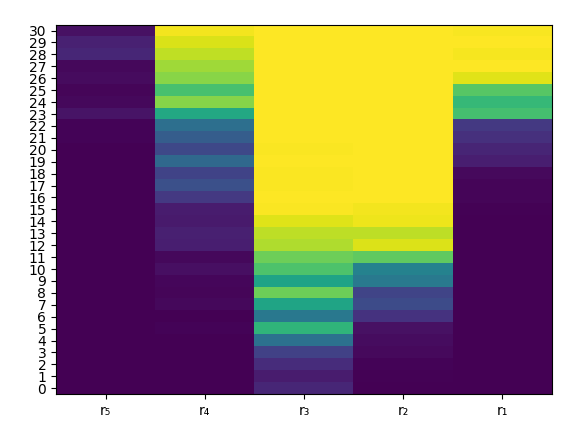
\includegraphics[width=0.48\textwidth]{Bilder/heatmap_1.png} 
\hspace{0.2 cm}
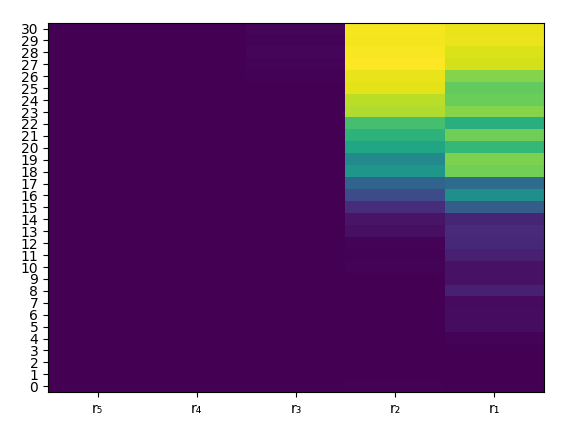
\includegraphics[width=0.48\textwidth]{Bilder/heatmap_2.png} 
\caption[]{Heatmap representing the models output. At the left image, an obstacle is predicted in front, with an edge pointing right towards the robot. The edge's distance is predicted to be about 0.6 m away from the robot. The right image predicts an obstacle at a distance of 1.80 m to the right, from the robot.}
\label{heatmap}
\end{figure}
\newpage

\section{Experimental Results \label{ExperimentalResults} }
This section summarizes the appendix to this project and the pipeline's development. The corresponding file for the appendix can be found under \path{ss20_lanz_2d_obstacle_avoidance/doc/thesis/Thesis_appendix.pdf}. The appendix lists all models trained as batches, where each batch contains models trained on a specific environment or with different parameters. Except for the pipeline's parameters, the appendix additionally lists results from the model's training and testing.\\

To guarantee a robust and successful process, suggestions from \cite{Goodfellow-et-al-2016} and \cite{DBLP:journals/corr/abs-1803-09820} are applied, as  discussed in \secref{monitoring}.  
One suggestion, which could be implemented directly, is to set up a functioning pipeline very early in the process to immediately discover and adjust functions or parameters, which cause errors or poor training performance. Even if one of the essential techniques to increase performance is to increase training data, the methods mentioned above were fundamental to acquire further knowledge about the model itself and the entire pipeline's execution. The training on small datasets to test the model's fitting ability, the recognition of duplicates at Feature Extraction or the correct prediction of images without obstacles are just a few examples where the techniques mentioned have been applied. The calculation of the Area Under the Curve and the visualization techniques gave a compelling insight into the model's performance, in a very exact and accurate in the former, and very intuitive, but extremely helpful in the latter.\\


The following subsection first gives a brief review of the pipeline development challenges and results and then discusses the pretraining and training phase. The first five batches trained are part of the pretraining phase, while the last batch, with knowledge applied from the pretraining, contains the final experimental results.

\subsection{Pipeline \label{pipeline}}
This section is about challenges faced while setting up the pipeline, during the early stages of the training process.\\

\textbf{Environment} As one of the requirements is to provide system independency, the project proposes a docker environment. A TensorFlow base image was chosen and extended with a ROS and TIAGo environment. As an interpreter, Python3 was used throughout the entire environment, which led to some ROS conflicts to solve. Using Python3 was rewarding in the end, as many libraries for machine learning like Scipy, Numpy, or Keras, could be used with up-to-date versions. Another challenge was to activate a graphical user interface within the docker environment for simulations, heatmaps, or graphs to be displayed or saved, or the implementation of functioning GPU support based on Tensorflow. Overall, it was very challenging, but rewarding to have all tools working and adjusted adequately for one environment.\\

\textbf{Data Acquisition} Setting up a robust and reliable Data Acquisition Controller was one of the most time-intense tasks for this project. During the entire process, functions had to be adjusted, rewritten, or extended to increase and guarantee a fully autonomous and safe data collection from different environments.\\

\textbf{Feature Extraction} As part of the concept is provided by \cite{nava2019learning}, the contribution for this part was mostly the proper implementation concerning the environment, architecture, and sensors used. Even if the concept was partially available, the effort to incorporate this stage within the pipeline was substantial. Additional functionalities, like error recognition mechanisms, a fully autonomous workflow, or the implementation of centralized parameter control, are among several extensions applied to this stage.\\

\textbf{Training} As well as for Feature Extraction, \cite{nava2019learning} provides a rough layout of the architecture setup with training scripts for datasets provided by the previous stage. As in Feature Extraction, the main challenge was the proper incorporation within the pipeline, with several new features and extensions applied as error recognition, autonomous workflow, file administration, and centralized parameter control.\\

\textbf{Performance Monitoring and Testing} To properly monitor the pipeline and have it run fully autonomous, several implementations were set up and iteratively adjusted, rewritten, or replaced. One complete replacement was the File Administration Class, which was considered too heavy and difficult to maintain after being used at the early stages. A subsequent version was created, easier to maintain, and use. It seemed practical to have a File Administration, logically store, name, and check files for consistency from the early stages upon, to save manual effort and time. Another handy tool was to implement custom error messages through all stages. This functionality was a beneficial debugging mechanism and provided useful hints of where changes had to be adapted. The visualization techniques in the form of videos and heatmaps were also beneficial to quantify a model's performance. It is much easier to look at a heatmap, instead of an array, and act upon its behavior. The entire manual testing, as described in \secref{sim_prototype}, could be done very effectively with heatmaps, representing predictions in real-time. Manual testing, compared with the Area under The Curve, could get additional insight into the model's behavior and performance.

\subsection{Pretraining and Debugging \label{pretraining}}

\textbf{Batch 1}\\
As in the chapter  11.3 of \cite{Goodfellow-et-al-2016}, which is about determining whether to gather more data or not, the author claims that if the validation set's performance is much worse than the training set's performance, the most effective way to increase a models performance is to gather more data for training. This concept can be observed in the first three models of Batch 1, which use a relatively small amount of input data. A more considerable amount of input returns better results for subsequent models on the validation set.\\

Another observation on Batch 1 is that most model's outer ranges, as $R_{1}$ or $R_{5}$, have inferior performance. As the outer range's performance is much lower overall models of Batch 1, in comparison to the center ranges, it appears reasonable to adjust parameters as the $laser range $, the $laser threshold$ or $safe_{d}$. Especially $safe_{d}$, which is a safe distance and determines the closest possible position the robot can approach an obstacle, impacts the gap of results among the center and outer ranges, as it directly influences how frequent the outer ranges are used. \figref{safe_d_adjustment} describes this concept, where a smaller value for $safe_{d}$ increases the use of the outer ranges.\\

A surprising result is delivered for Model 13 from Batch 1. The model's quality decreases over the quality of model 5, although a much more considerable amount of images is provided for training.\\

The learning rate for all models, except Model 14 and 15, is kept at 0.0002. As suggested by \cite{DBLP:journals/corr/abs-1803-09820}, and discussed in \secref{hyperparameters}, the learning rate can be increased if a model underfits. This concept is applied for Dataset 13 with the results of Model 14, which seems to be more stable at the validation loss. A further increase in the learning rate on the same dataset drastically decreased performance. This can be seen at the results of Model 15 and at \figref{learning_rate_test}.\\

The recognition of unknown obstacles performs poorly over the entire batch. Especially distances are not interpreted correctly. Ranges, on the other hand, are correctly predicted in some cases.\\

Distance accuracy also performs relatively low. It can be observed that with increasing distances of obstacles, their prediction gets more accurate. This behavior seems to be an issue of the parameter $laserthreshold$ and $safe_{d}$, which are adjusted on future batches.

\vspace{0.2 cm}
\begin{figure}[h]%[htbp]
\centering
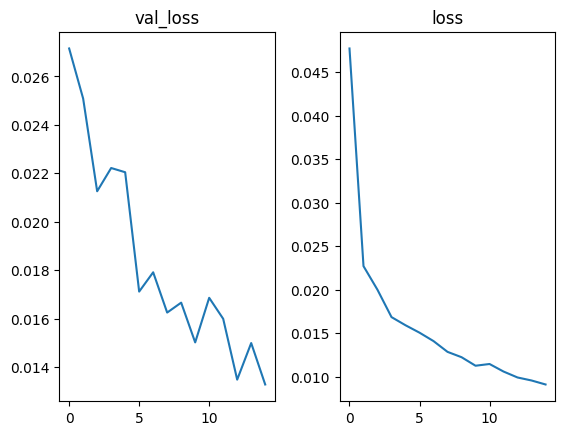
\includegraphics[width=0.30\textwidth]{3_models/models_13/graph_13.png}
\hspace{0.2 cm}
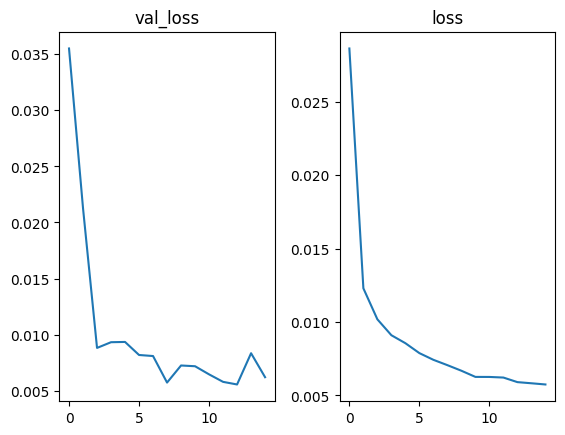
\includegraphics[width=0.30\textwidth]{3_models/models_14/graph_14.png}
\hspace{0.2 cm}
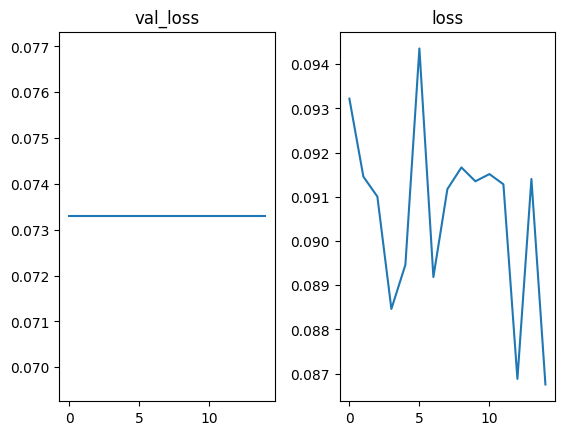
\includegraphics[width=0.30\textwidth]{3_models/models_15/graph_15.png}
\caption[]{Learning rate test with an increasing value run on three models. The last model's performance, drastically decreases.}
\label{learning_rate_test}
%\vspace{-50pt}
\end{figure}

Empty instances are recognized through all models except the last model of Batch 1. As the problem of not recognizing instances without obstacles has already been solved during debugging, this behavior is expected.\\

The correct recognition of ranges gradually increases with the number of images used. Model 5 provides the most accurate predictions of ranges for this batch.\\

Looking at the Area Under the Curve results, one might consider Model 4 as the winner for Batch 1. The reality is that Model 4 performs rather poorly on the simulation test for correct distances. The model seems to be too sensitive to see obstacles that are further away than the recording distance. As the Area Under the Curve is calculated on the validation set, it lacks the knowledge of obstacles further away than the recording distance, as all recordings on the validation set are within the recording distance range. Therefore, Model 5, instead of Model 4, is set as the winner for Batch 1. Model 5 is given a more considerable amount of training data, which reduces this too high sensitivity of Model 4, and allows it to generalize more efficiently.\\

\begin{figure}[H]%[htbp]
\centering
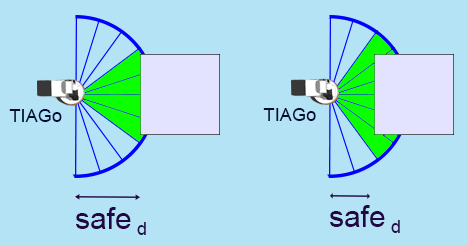
\includegraphics[width=1\textwidth]{Bilder/safe_d.png} 
\caption[]{Concept of the effect on ranges used by changing the parameter $safe_{d}$.}
\label{safe_d_adjustment}
\end{figure}


\textbf{Batch 2}\\
As this batch's environment provides a substantially more considerable variety of obstacles, the overall performance somewhat decreased compared to the results of Batch 1. As the average number of images extracted per obstacle decreases due to a greater variety, this behavior seems trivial. This side effect can be countered to increase the input as in Model 11, which provides the best results with 30000 images in the dataset. The greater variety has advantages as well when it comes to recognizing unknown obstacles, which also makes sense, as the probability of an unknown obstacle to be more similar to a known obstacle is higher if the variety is more significant, to begin with.\\

As the environment's complexity heavily increased, several adjustments are necessary to guarantee a robust and fully autonomous gathering of data. At the early stages, this environment caused the robot to get frequently stuck in a loop, which could be fixed by setting some timeouts if a particular state would not change.\\

\textbf{Batch 3}\\
To increase the side ranges performance, as discussed analyzing Batch 1, and in \figref{safe_d_adjustment}, the $laser threshold$ and  $safe_{d}$ are decreased for this batch. A low value like 0.2 for $safe_{d}$ causes collisions at certain angles of this environment's brick wall obstacle. The value can be set to 0.35 without the robot crashing.\\

The overall performance of high input models is satisfying but not perfect yet. It can be observed that the performance of the outer ranges averagely increased in comparison to Batch 1 or Batch 2. Especially Models 26, 27, and 28 provide pretty decent results. Also, the distance accuracy improves for the middle part, which is from 1 to 2 meters. For very close obstacles, the distance prediction is still not very accurate.\\

\textbf{Batch 4}\\
For this batch, the recording distance is changed. As the camera used for this simulation can recognize obstacles up to 8 meters, it might be rewarding to take advantage of that. As intermediary positions, a value of 81. This change increases the number of images recorded to about 154, for each bagfile. The increase of recording distance has several impacts. It requires a more considerable amount of computational resources, like the Neural Network's output instead of (1,155) for 31 intermediary positions increases to (1,405) for 81 intermediary positions. The time to create a dataset or train a model substantially increases.\\

A more considerable recording distance aims to make the model less sensitive to objects further away than the recording distance. This problem is discussed analyzing Model 4 at Batch 1.\\

While the first models' results are expected with respect to the rest of the pipeline results, the last model performs very poorly. Model 39 fails on all tests, like the Area Under the Curve, as well as on the manual simulation. More tests with more significant computational resources could probably be rewarding.\\

\textbf{Batch 5}\\
As some results of Batch 4 are shallow, and further analysis concludes that the cause might be an implementation error, the selection range, as well as the distribution of intermediary position is adjusted for this batch.\\ 

The selection range is a setting at Feature Extraction, which limits possible intermediary positions around a specific threshold or uses the entire bagfiles odometry information to find intermediary positions as described in \secref{finding_positions}.\\

The distribution of intermediary positions is a value which distributes the intermediary positions set over the recording distance. As the intermediary positions are set in decimeters, for a recording distance of 4 meters, 40 intermediary positions are chosen. If intermediary positions are applied as

\begin{equation}
\label{eqn:14} 
f(n) = \frac{n}{10}
\end{equation}

it would cause immense distances to get insufficient weight for training. The results can be seen at Batch 5, where all models have a deficient performance for distances starting at about 3.5 meters. For the final training, the denominator of the equation \ref{eqn:14} will be set higher. This change will shrink the intermediary positions within the recording distance and lead to more accuracy at distances that are further away.

\subsubsection{Conclusion Pretraining \label{conclusion_pretraining}}
The following main observations about the model's performances can be concluded from the pretraining phase. For each result, a proper solution is suggested and applied, to increase the model's performance further:

\begin{itemize}
\item Low results on the outer ranges over all batches
\item No distance recognition of unknown obstacles overall batches
\item Low performance of distance recognition, especially to distances in the immediate vicinity and the center of the prediction
\end{itemize}

\textbf{Outer ranges}\\
Increasing the results of the outer ranges is already discussed in the analysis of Batch 1. A decrease of the value $d_{safe}$ is suggested at this step. Another possibility is to increase the density of the environment. That change would lead to the outer ranges being used more frequently.\\

\textbf{Unknown obstacles}\\
Increasing the variety of obstacles would increase the probability of unknown obstacles to be recognized. 

\textbf{Distance recognition}\\
As the predictions for distances are unreliable overall batches, a sever calculation bug can be fixed after extensive analysis of the pipeline's results. The intermediary positions distribution parameters, over the recording distance, are adjusted, at Feature Extraction.\\

Interestingly, the performance issues mentioned are rather caused by calculation or implementation errors, instead of training parameters set wrong. This behavior can be concluded from the prediction being accurate for some models or some parts of the models. By some parts, a specific range or distance range is considered. The next chapter summarizes models trained, with knowledge and insight obtained from the pretraining phase.
\newpage

\subsection{Final Results \label{final_results}}
In this chapter, the final testing results are presented. Batch 6 is individually trained and contains seven models with images ranging from 2400 to 13840. Batch 6 can further be split into two sets of models, where the first set (Model 47, 48, 49, and 62) is trained on a recording distance of 4 meters, and the second set (Model 59, 60, and 61) is trained on a recording distance of 3.5 meters. As mentioned in \secref{conclusion_pretraining}, this batch is trained upon experience and knowledge gained from the pretraining phase.\\

By comparing the two sets, the overall performance is slightly better on the first. \figref{final_set_1} displays the gradual increase of Set 1, increasing the number of images from 3440 to 13840.

\begin{figure}[H]%[htbp]
\centering
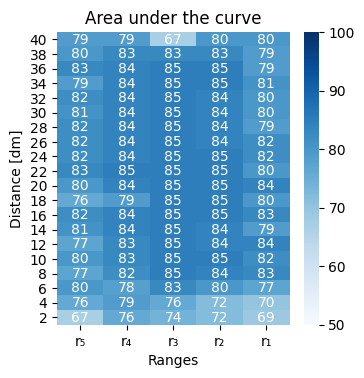
\includegraphics[width=0.31\textwidth]{4_plots/plots_47/AUC_47.png}
\hspace{0.2 cm}
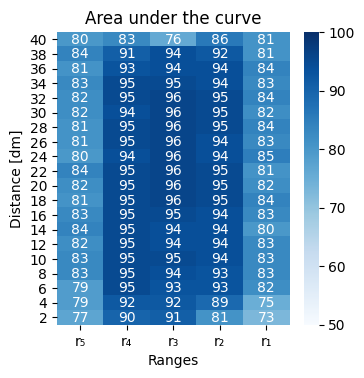
\includegraphics[width=0.31\textwidth]{4_plots/plots_48/AUC_48.png}
\hspace{0.2 cm}
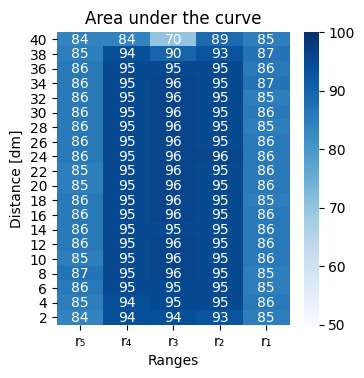
\includegraphics[width=0.31\textwidth]{4_plots/plots_49/AUC_49.png}
\caption[]{Comparsion of Model 47, 48 and 49, with a gradual increase of performance, relative to the increase of training data.}
\label{final_set_1}
\end{figure}

The following sub-chapter further compares the two best of all models. The manual testing results, which can be seen in the appendix in Table 6, show equally good results for both. Model 49 is further used to create a video displaying the results of its performance. The video can be obtained within the repository on the following path:
\path{ss20_lanz_2d_obstacle_avoidance/doc/thesis/Videos/Final_video.mkv} 

\subsubsection{Model 49 \label{model_49}}
One of the best of all models trained for this project is Model 49, which displays high accuracy on all tests. \figref{best_model_49} displays the Area under the Curve, the Training vs. the Validation loss, and a graph for the Generalization Error.\\

\textbf{AUC} The results of the Area under the Curve for Model 49 are among the best of all models trained. The outer, but especially the inner ranges, averagely display results up to 95. As the parameter $safe_{d}$ already had been at a minimal value, the model's outer range quality could be further increased by increasing the density of the environment as discussed in \secref{conclusion_pretraining}.\\

\textbf{Validation vs. Training loss} By looking at the second image of \figref{best_model_49}, the training loss is lightly lower than the validation loss, which indicates the model to be lightly overfitting. The validation loss, furthermore displays the desired horizontal line, as described in \cite{DBLP:journals/corr/abs-1803-09820}. This desired horizontal line can also be observed, looking at the results of Model 62 of Batch 6 in the appendix.\\

\textbf{Generalization Error} This plot is calculated by subtracting the training loss from the validation loss. The graph first increases and then stays in a horizontal form at around 0.01.

\begin{figure}[H]%[htbp]
\centering
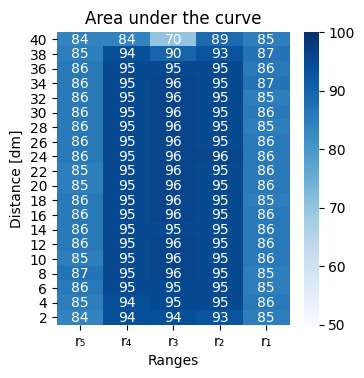
\includegraphics[width=3.8cm, height=4cm]{4_plots/plots_49/AUC_49.png}
\hspace{0.2 cm}
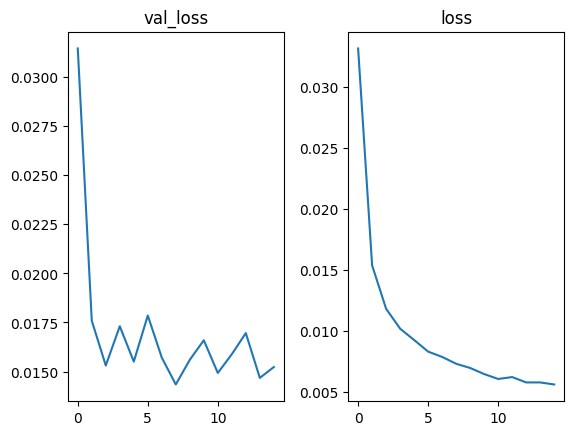
\includegraphics[width=4.8cm, height=4cm]{3_models/models_49/graph_49.png}
\hspace{0.2 cm}
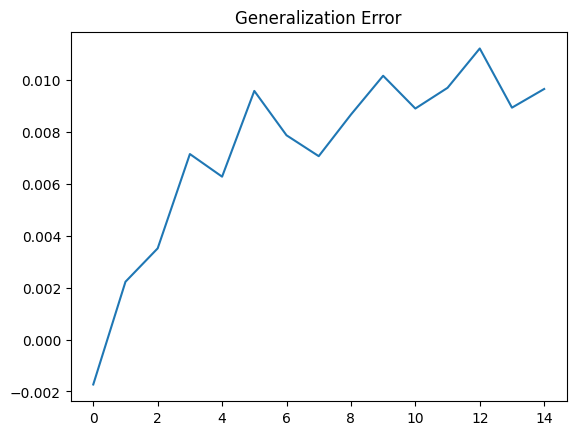
\includegraphics[width=4.8cm, height=4cm]{3_models/models_49/gen_loss_49.png}
\caption[]{Result plots for Model 49 of Batch 6.}
\label{best_model_49}
\end{figure}

\subsubsection{Model 62 \label{model_62}}
Another model worth mentioning is Model 62 of Batch 6. This model is trained on the same dataset as Model 49, with the difference of 30 epochs instead of 15 used.\\

\figref{best_model_62} displays the results of Model 62. While the results for the Area under the Curve nearly stays the same, the generalization error can be further decreased to about 0.004. This is due to a better performance of the validation loss, which fluctuates around 0.01. 

\begin{figure}[H]%[htbp]
\centering
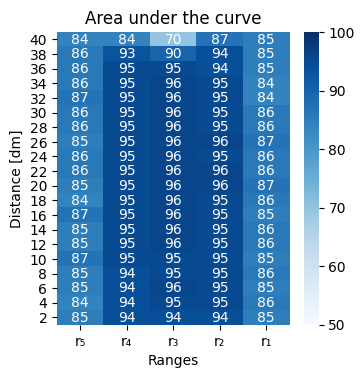
\includegraphics[width=3.8cm, height=4cm]{4_plots/plots_62/AUC_62.png}
\hspace{0.2 cm}
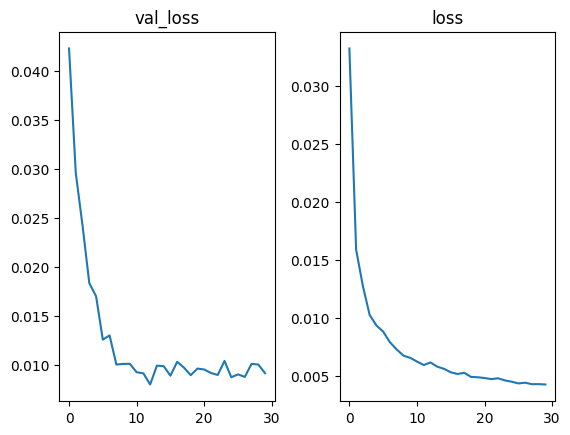
\includegraphics[width=4.8cm, height=4cm]{3_models/models_62/graph_62.png}
\hspace{0.2 cm}
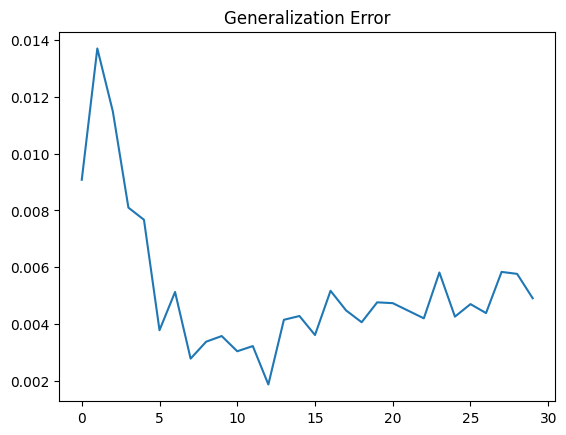
\includegraphics[width=4.8cm, height=4cm]{3_models/models_62/gen_loss_62.png}
\caption[]{Result plots for Model 62 of Batch 6.}
\label{best_model_62}
\end{figure}

\section{Conclusion \label{Conclusion} }
This Bachelor thesis presented a self-supervised Machine Learning pipeline, used to develop an obstacle avoidance controller, which can maneuver an environment, with images as input alone.\\

The pipeline was implemented platform-independent, fully autonomous over all stages, with error recognition, consistency, and documentation functionalities. Each pipeline stage further provides excellent flexibility, maintainability, and possibilities to adjust or extend parameters by a centralized control mechanism easily.  The suggestion by \cite{Goodfellow-et-al-2016} to implement a functioning pipeline, very early in the training process, was beneficial to improve the project's performance early and achieve an efficient training of accurate models, iteratively.\\

The extensive analysis of the pre-training results provided a valuable and rewarding insight into the pipeline's performance, leading to applying the acquired knowledge for final training. The final results presented some efficient models, which underline the concept's effectiveness. The project shows that it is possible to gather data effectively, relate the acquired camera data with short-range information to train a model on the developed dataset, test the model and iteratively increase the model's performance. The final model can then be efficiently used to test and implement an obstacle avoidance controller, which can maneuver a simulation environment, by images from a camera alone.\\

The implementation also displayed disadvantages, which derive from the fact that just one camera is used as input. Future research might be rewarding to extend the current implementation with side cameras equipped to provide a more accurate controller, especially for the robot's outer ranges.


\begin{comment} 
\nocite{coulouris00, coulouris02} 
\end{comment} 

\addcontentsline{toc}{section}{References} 
\bibliographystyle{alphadin} 
\bibliography{Literature_en} 

\end{document} 


